\chapter{Specific Requirements}

\section{External Interface Requirements}

\subsection{User Interfaces}

\subsection{Hardware Interfaces}
DREAM is a web application, as such each user should own a device capable of installing a modern browser. Form factor of the device does not matter, as DREAM application is fully responsive.

\subsection{Software Interfaces}
A modern browser is necessary to use the system. DREAM supports most major browsers. However, in order to ensure full functionality, below is a list of browsers that are fully supported.
\begin{itemize}
    \setlength\itemsep{0em}
    \item Google Chrome
    \item Firefox
    \item Safari
    \item Microsoft Edge
    \item Opera
\end{itemize}
User should always update their browser to keep up with security, compatibility and functionality.

\subsection{Communication Interfaces}
To perform any kind of operation using the system, a stable internet connection is required (Wi-Fi or cellular).

\section{Functional Requirements}

\begin{longtable}{@{}p{0.06\linewidth} p{0.88\linewidth}}
		\toprule
		\textbf{ID}   & \textbf{Requirement}\\
		\midrule
		
		%Authentication
		\textbf{R1.} & The system must uniquely identify each user by his e-mail. \\
		\textbf{R2.} & The system must allow an unregistered user to create an account with a chosen role. \\
		\textbf{R3.} & The system must ensure that an agronomist chooses the area of responsibility during the registration process. \\
		\textbf{R4.} & The system must ensure that a farmer inserts his farm data during the registration process.\\
		\textbf{R5.} & The system must ensure that two casual farm visits are scheduled for each year of the farm's existence.\\
		\textbf{R6.} & The system must allow a registered user to log in to the application. \\
		\textbf{R7.} & The system must allow a registered user to reset his password. \\
		\textbf{R8.} & The system must allow a logged-in user to sign out of the application. \\
		\textbf{R9.} & The system must allow a registered user to delete his account. \\
		
		%Policy maker
		\textbf{R10.} & The system must allow a policy maker to assign a note to a farmer.\\
		\textbf{R11.} & The system must ensure that every farmer initially has a neutral note.\\
		\textbf{R12.} & The system must have a list of predefined farmer's problem types.\\
        \textbf{R13.} & The system must allow a policy maker to specify a problem type when assigning a negative note.\\
        \textbf{R14.} & The system must ensure that a farm is visited more often in the event of any problems.\\
        \textbf{R15.} & The system must have a specified number of additional visits caused by each predefined problem type.\\
        \textbf{R16.} & The system must ensure that only the most recently specified problem type is taken into account when determining the number of visits.\\
		\textbf{R17.} & The system must ensure that an automatic help request followed by additional farm visits are created, if a farmer receives a negative note.\\
		\textbf{R18.} & The system must ensure that all the additional farm visits created due to obtaining a negative note are deleted after a farmer's negative note is updated with a positive or a neutral one.\\
		\textbf{R19.} & The system must allow a policy maker to see a list of all farmers in Telangana.\\
		\textbf{R20.} & The system must allow a policy maker to see a list of all farmers with a specific note.\\
		\textbf{R21.} & The system must allow a policy maker to see a list of all farmers in a given mandal.\\
		\textbf{R22.} & The system must allow a policy maker to find a farmer's summary by his name and surname.\\
		\textbf{R23.} & The system must allow a policy maker to see a farmer's summary.\\
		
		%Farmer
		\textbf{R24.} & The system must allow a farmer to see his own farmer's summary.\\
		\textbf{R25.} & The system must allow a farmer to see personalized suggestions.\\
		\textbf{R26.} & The system must allow a farmer to manage his monthly production data.\\
		\textbf{R27.} & The system must allow a farmer to see a list of help requests created by him.\\
		\textbf{R28.} & The system must allow a farmer to find a help request created by him by the topic.\\
		\textbf{R29.} & The system must allow a farmer to see a specific help request created by him.\\
		\textbf{R30.} & The system must allow a farmer to delete a specific help request created by him.\\
		\textbf{R31.} & The system must allow a farmer to create a new help request.\\
		\textbf{R32.} & The system must allow a farmer with a positive note to see a list of all help requests in his mandal.\\
		\textbf{R33.} & The system must allow a farmer with a positive note to find a help request in his mandal by the topic.\\
		\textbf{R34.} & The system must allow a farmer with a positive note to see a specific help request in his mandal.\\
		\textbf{R35.} & The system must allow a farmer with a positive note to respond to a specific help request in his mandal.\\
		\textbf{R36.} & The system must allow a farmer with a positive note to delete a help response, only if it was created by him.\\
		\textbf{R37.} & The farmer is able to see farmer's summary of a farmer with a negative note whose help request he received. \\
		\textbf{R38.} & The system must allow a farmer to see a list of all forum threads in Telangana.\\
		\textbf{R39.} & The system must allow a farmer to find a forum thread by the topic.\\
		\textbf{R40.} & The system must allow a farmer to see a specific forum thread with its comments.\\
		\textbf{R41.} & The system must allow a farmer to create a comment in a forum thread.\\
		\textbf{R42.} & The system must allow a farmer to delete a comment in a forum thread, only if it was created by him.\\
		\textbf{R43.} & The system must allow a farmer to create a forum thread.\\
		
		%Agronomist
		\textbf{R44.} & The system must allow an agronomist to manage his area of responsibility.\\
		\textbf{R45.} & The system must allow an agronomist to see the list of suggestions for mandals in his area of responsibility.\\
		\textbf{R46.} & The system must allow an agronomist to manage the list of suggestions for mandals in his area of responsibility.\\
		\textbf{R47.} & The system must allow an agronomist to see a list of all farmers in his area of responsibility.\\
		\textbf{R48.} & The system must allow an agronomist to see a list of all farmers with a specific note in his area of responsibility.\\
		\textbf{R49.} & The system must allow an agronomist to see a list of all farmers in a given mandal in his area of responsibility.\\
		\textbf{R50.} & The system must allow an agronomist to find a farmer's summary in his area of responsibility by his name and surname.\\
		\textbf{R51.} & The system must allow an agronomist to see a farmer's summary in his area of responsibility.\\
		\textbf{R52.} & The system must allow an agronomist to see a list of all help requests in his area of responsibility.\\
		\textbf{R53.} & The system must allow an agronomist to find a help request in his area of responsibility by the topic.\\
		\textbf{R54.} & The system must allow an agronomist to see a specific help request in his area of responsibility.\\
		\textbf{R55.} & The system must allow an agronomist to respond to a specific help request in his area of responsibility.\\
		\textbf{R56.} & The system must allow an agronomist to delete a help response, only if it was created by him.\\
		\textbf{R57.} & The system must allow an agronomist to see his daily plans.\\
		\textbf{R58.} & The system must allow an agronomist to submit a daily plan's execution state, by rejecting or confirming each visit, on the same date or after the daily plan's date has passed. \\
		\textbf{R59.} & The system must allow an agronomist to provide a comment for a visit he is confirming.\\
		\textbf{R60.} & The system must ensure that after an agronomist submits his daily plan, for all the causal visits marked as confirmed, new ones are created in approximately half of a year.\\
		\textbf{R61.} & The system must allow an agronomist to delete a visit before its date.\\
		\textbf{R62.} & The system must ensure that a deleted visit is marked as rejected.\\
		\textbf{R63.} & The system must ensure that in case of rejecting a casual visit, a new one is created in maximally 5 days.\\
		\textbf{R64.} & The system must allow replanning any different visit than a casual one without any constraints.\\
		
% 		External systems
		\textbf{R65.} & The system must read and update weather forecasts every day. \\
		\textbf{R66.} & The system must read and store data from humidity sensors every day. \\
		\textbf{R67.} & The system must read and store data from water irrigation systems every day. \\

        
		
	\bottomrule
\end{longtable}

\subsection{Use cases}
\begin{figure}[H]
    \centering
    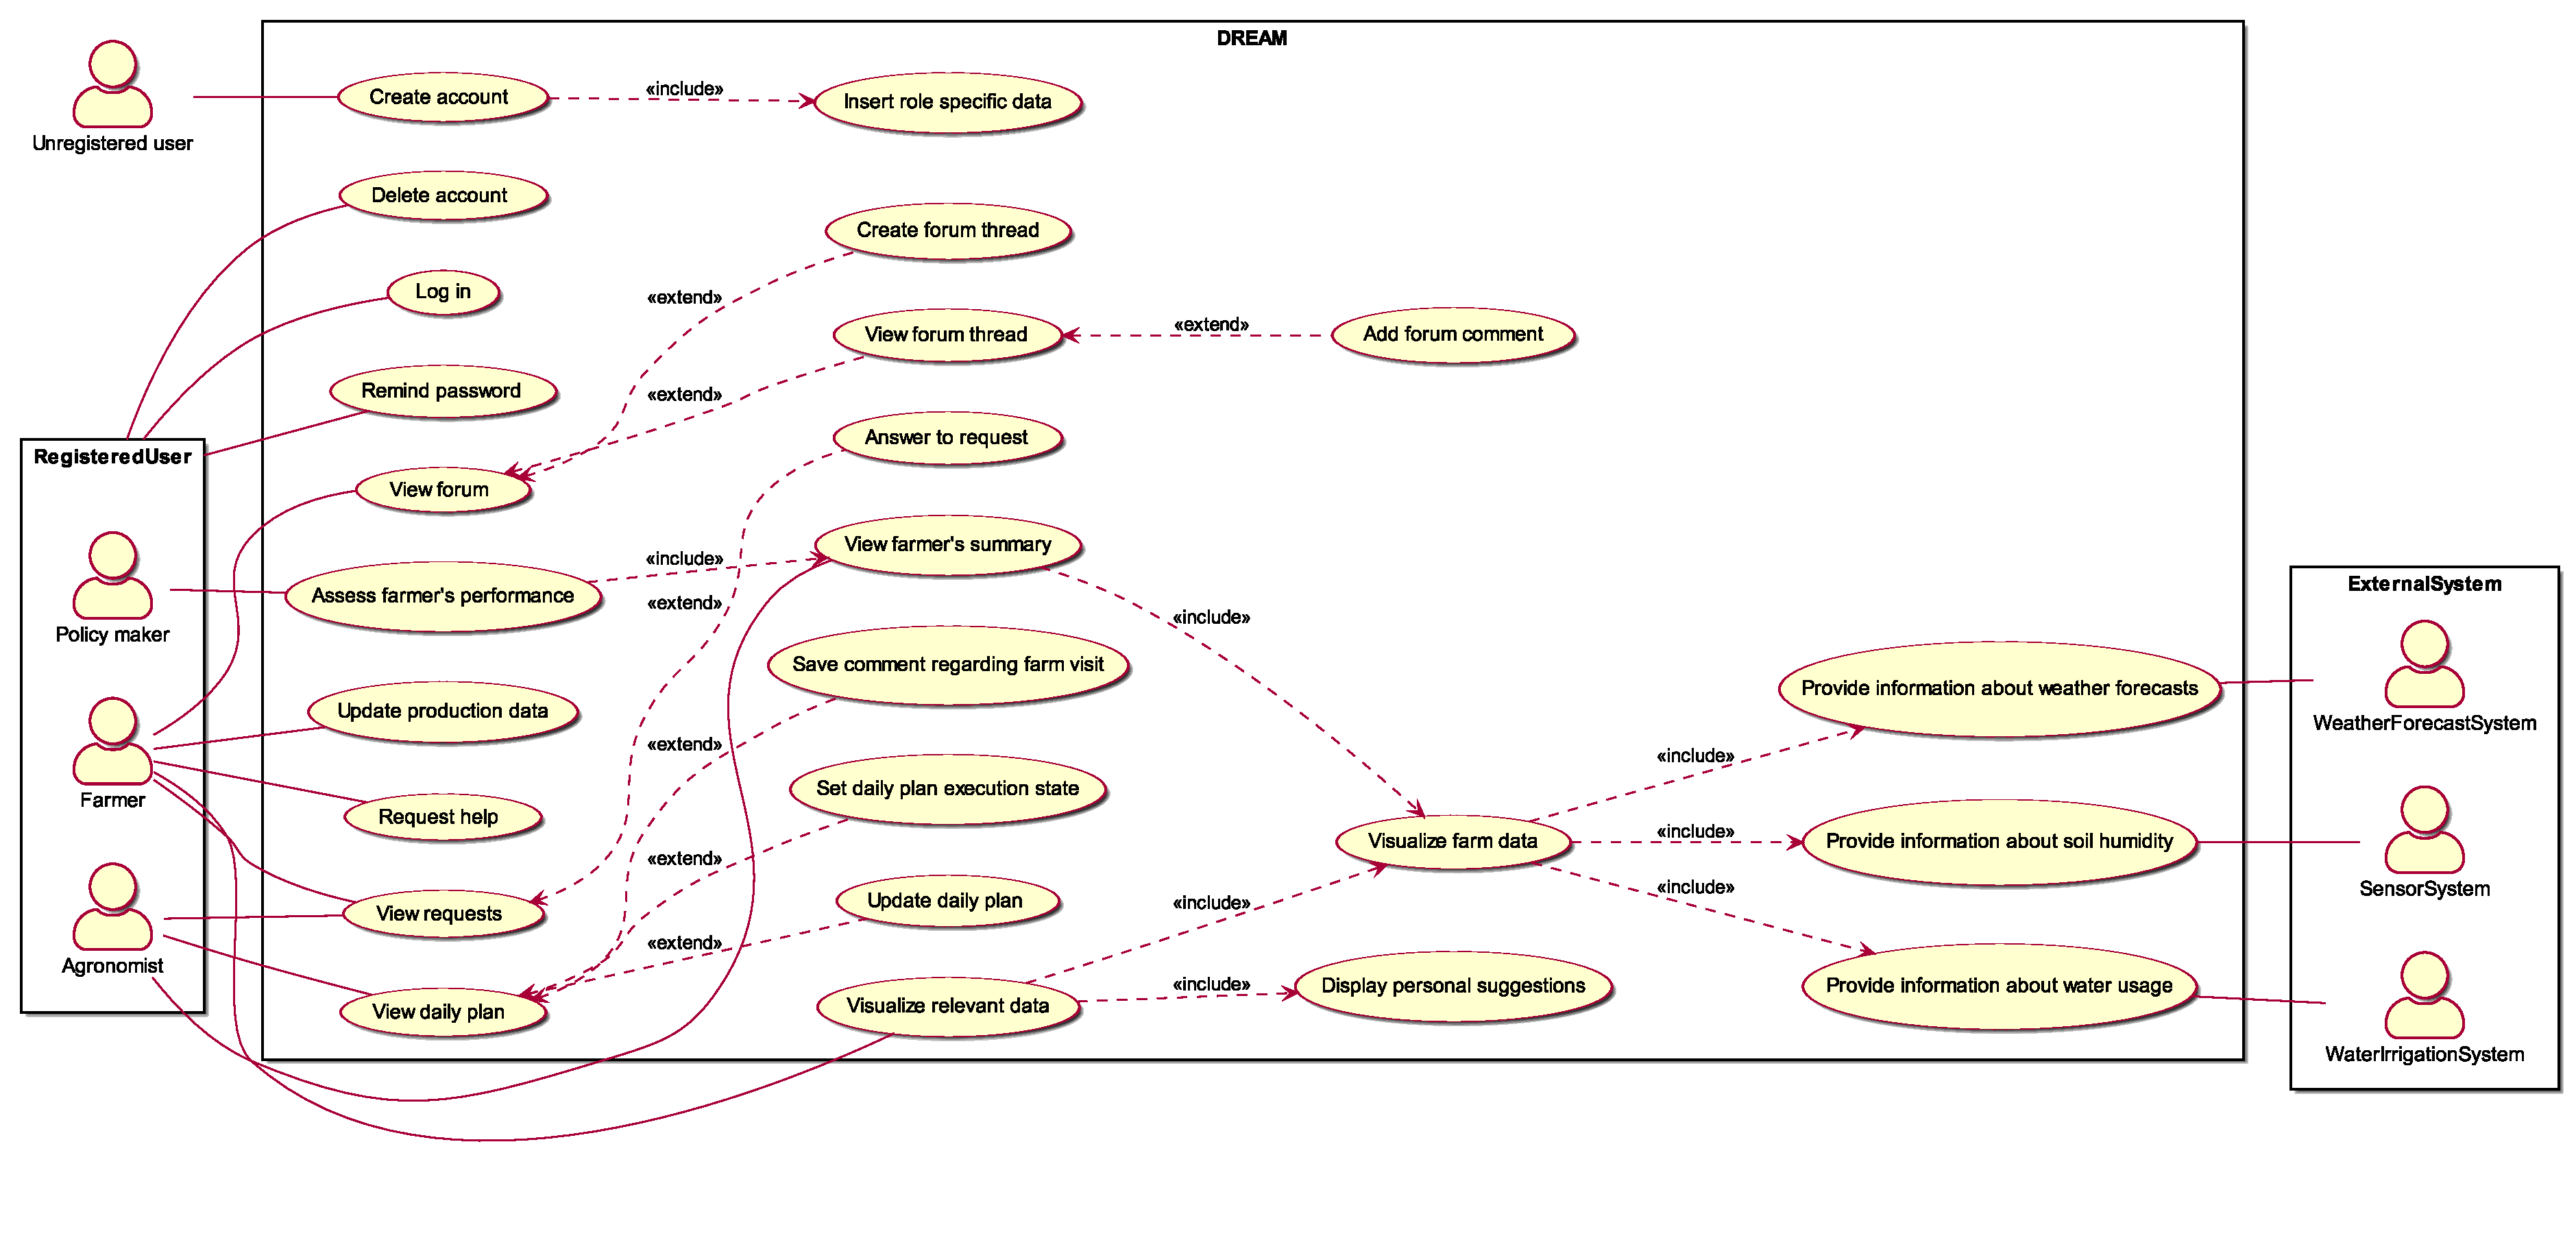
\includegraphics[width=0.92\textheight, keepaspectratio, origin=c, angle=90]{diagrams/use_case}
    \caption{Use case diagram.}
    \label{fig:uc_diagram}
\end{figure}

% Definition of use case diagrams, 
% use cases and associated sequence/activity diagrams, 
% and mapping on requirements

Given the great number of different use cases, the descriptions of only the most important ones are provided below.

\begin{table}[H]
	\begin{tabular}{@{}p{0.25\linewidth} p{0.72\linewidth}@{}}
		\toprule
		\textbf{Name}               & Create account \\
		\midrule
		\textbf{Actors}             & Unregistered user \\
		\midrule
		\textbf{Goals}              & G1, G2, G3, G4, G5, G6 \\
		\midrule
		
		\textbf{Entry conditions}   & \begin{itemize}[leftmargin=.4cm,noitemsep,topsep=0pt,before=\vspace{-3mm},after=\vspace{-4mm}]
		    \item The unregistered user, who wants to create an account, is  on the welcome screen of the application.
		\end{itemize}\\
		\midrule
		
		\textbf{Flow of events}     & \begin{enumerate}[leftmargin=.4cm,noitemsep,topsep=0pt,before=\vspace{-3mm},after=\vspace{-4mm}]
		    \item The unregistered user clicks on \textit{Create account} button on top.
		    \item The application shows a form with role-irrelevant data (email, name, surname and password) to fill and a dropdown to choose the role.
		    \item The unregistered user fills the form and selects a role.
		    \item If a role of a farmer was chosen, the application shows another part of the form with text fields related to farm data to be filled.
		    \item If a role of an agronomist was chosen, the application shows another part of the form that asks to manage mandals in the agronomist's area of responsibility.
		    \item The unregistered user fills role-related data if there is any.
		    \item If a role of a farmer was chosen, the system creates a farm for a farmer and two casual visits, which will take place in the following year, starting from the current date.
		    \item If a role of an agronomist was chosen, the system adds selected mandals to the agronomist's area of responsibility.
		    \item The unregistered user clicks on \textit{Create account} button.
		    \item The application creates a new user.
		    \item The application shows a message indicating successful registration.
		    \item The application shows the log in screen.
		\end{enumerate}\\
		\midrule
		\textbf{Exit conditions}    & A new user is created in the system. From now on, the credentials entered during the registration process can be used to log in to the application. \\
		\midrule
		
		\textbf{Exceptions}         & \begin{itemize}[leftmargin=.4cm,noitemsep,topsep=0pt,before=\vspace{-3mm}]
		   \item The unregistered user cancels the operation, clicking on a Cancel button or a cross in the top right corner of the pop-up.
		\end{itemize}
		The application shows the welcome screen.
		\begin{itemize}[leftmargin=.4cm,noitemsep,topsep=0pt]
		   \item The user with the given email address already exists. 
		\end{itemize}
		The application shows a message explaining that the user with given email already exists.
		\begin{itemize}[leftmargin=.4cm,noitemsep,topsep=0pt]
		   \item Some part of the form was not filled or was filled incorrectly.
		\end{itemize}
		The application shows a message explaining the type of error made by the user.
	    \begin{itemize}[leftmargin=.4cm,noitemsep,topsep=0pt]
		   \item The application is not able to create a new user in step 10.
		\end{itemize}
		The application shows a message indicating a possible cause of the error.
	    \\\bottomrule
	\end{tabular}
	\caption{Use case description: Create account.}
\end{table}

\begin{figure}[H]
    \centering
    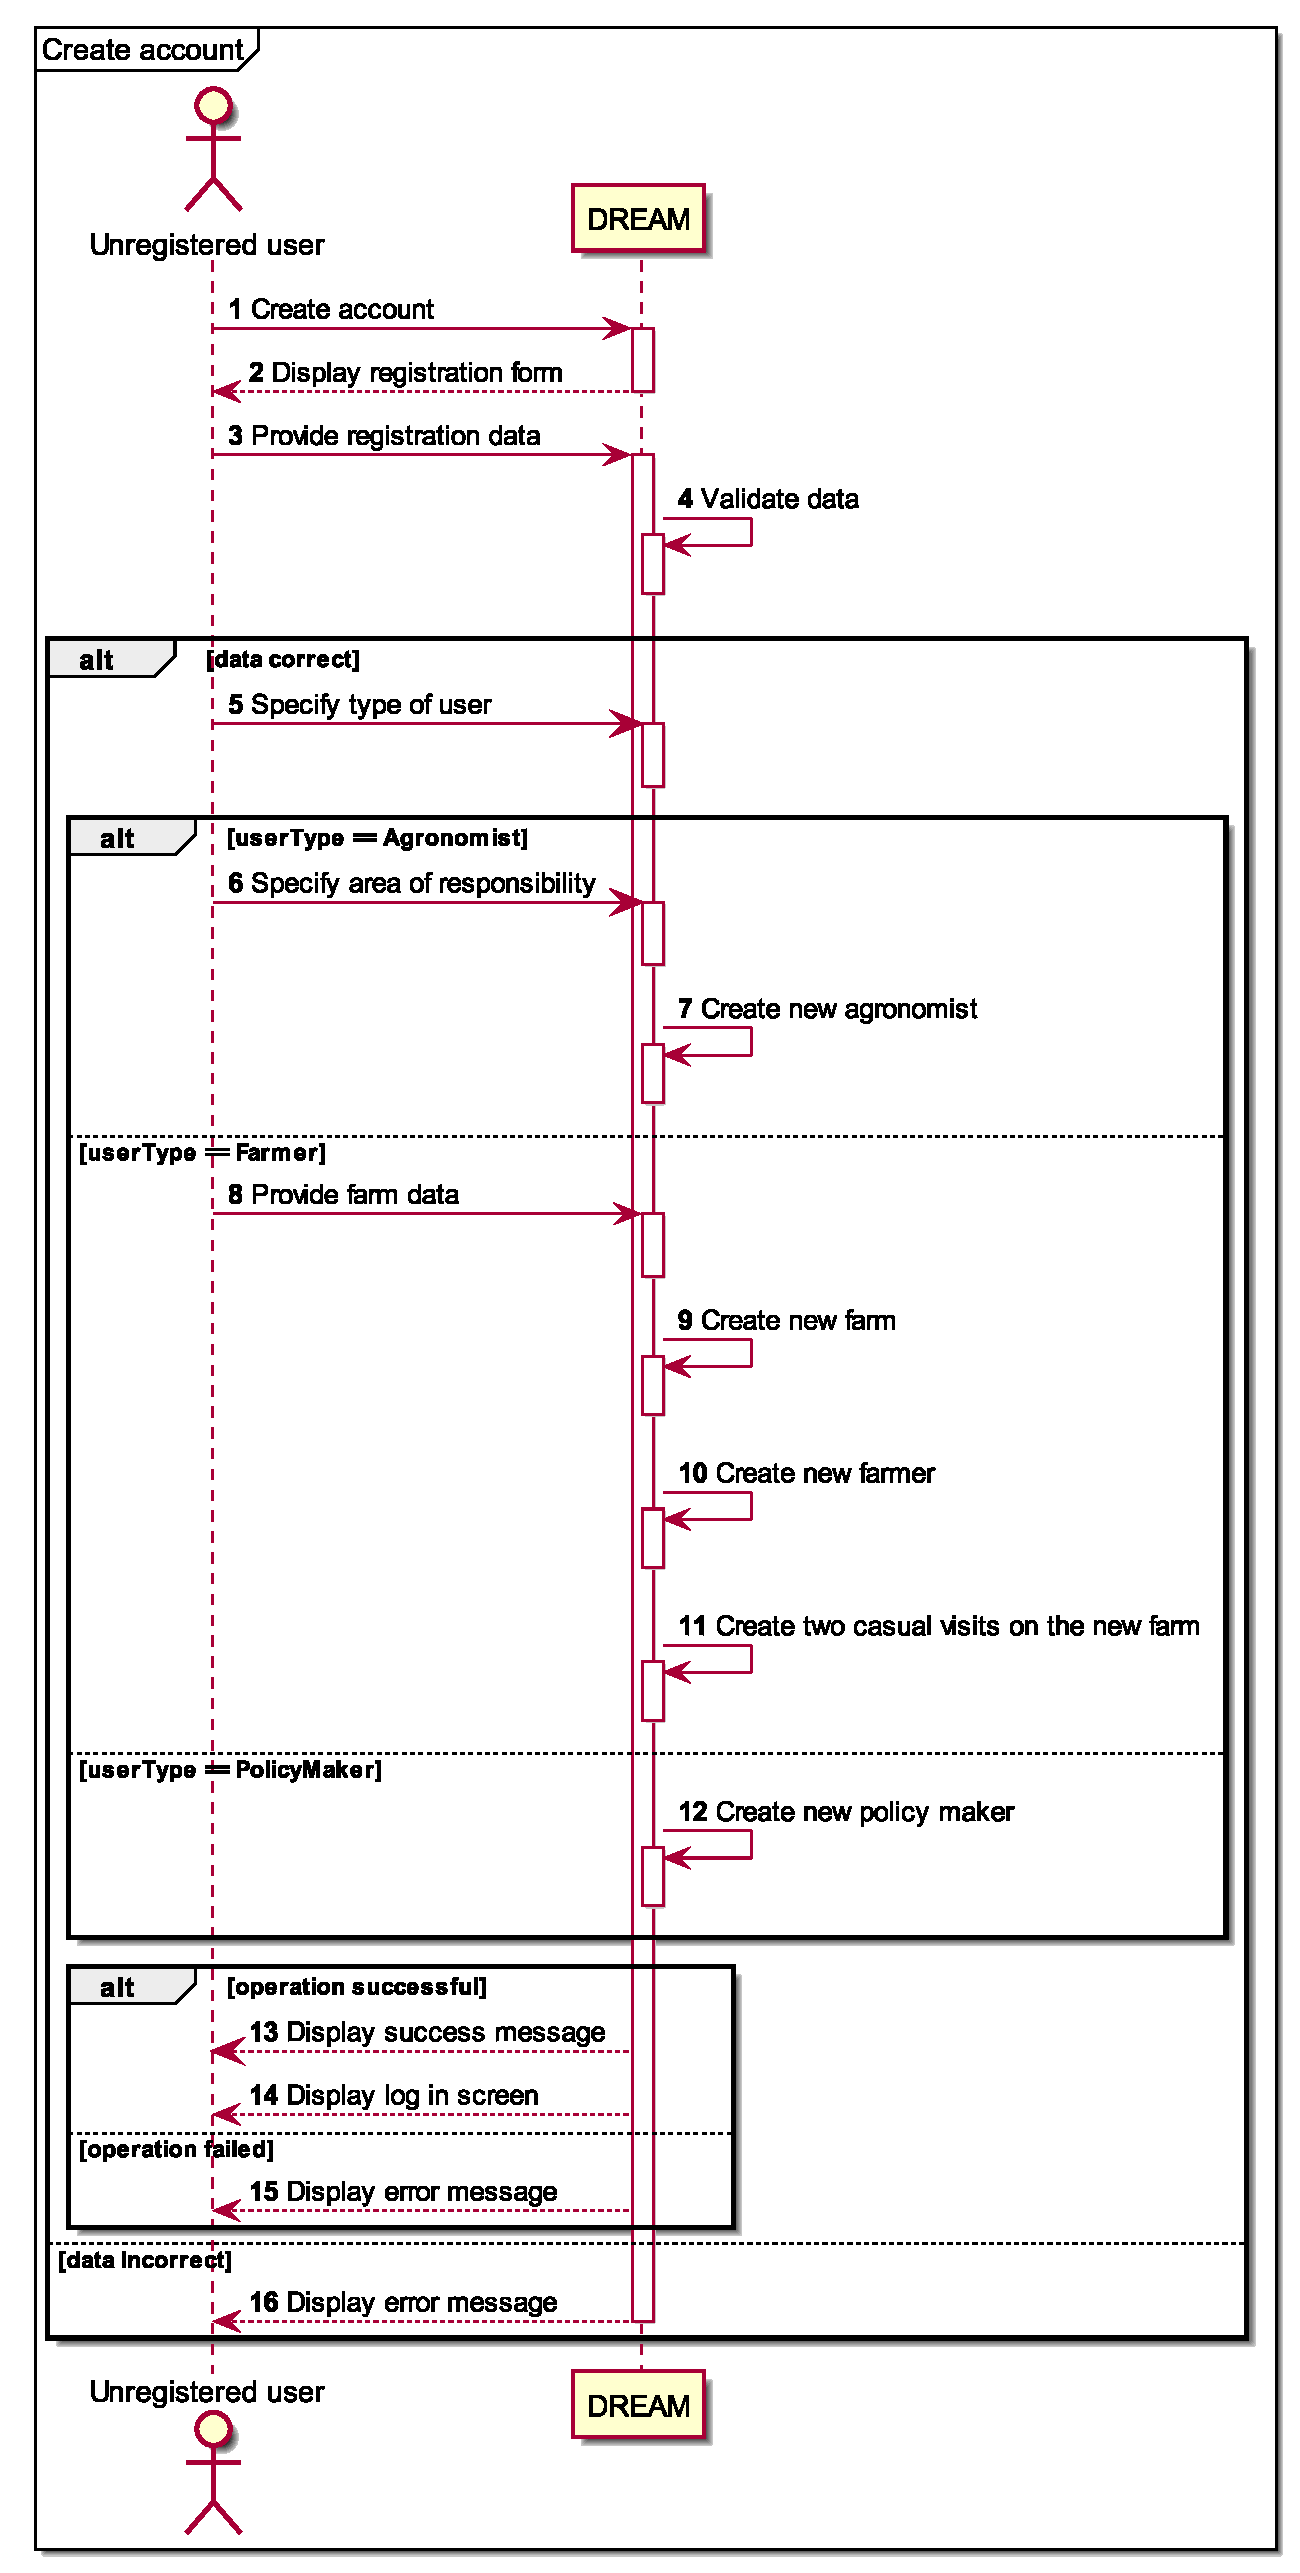
\includegraphics[scale=0.5, keepaspectratio, origin=c]{diagrams/sequence/create_account}
    \caption{Sequence diagram presenting the process of creating a new user account.}
    \label{fig:sd_create_account}
\end{figure}

\begin{table}[H]
    \centering
	\begin{tabular}{@{}p{0.25\linewidth} p{0.72\linewidth}@{}}
\toprule
		\textbf{Name}               & Log in\\
		\midrule
		\textbf{Actors}             & Policy maker, Agronomist, Farmer\\
		\midrule
		\textbf{Goals}              & G1, G2, G3, G4, G5, G6 \\
		\midrule
		
		\textbf{Entry conditions}   & \begin{itemize}[leftmargin=.4cm,noitemsep,topsep=0pt,before=\vspace{-3mm},after=\vspace{-4mm}]
		    \item The user, who wants to log in, is  on the welcome screen of the application.
		\end{itemize}\\
		\midrule
		
		\textbf{Flow of events}     & \begin{enumerate}[leftmargin=.4cm,noitemsep,topsep=0pt,before=\vspace{-3mm},after=\vspace{-4mm}]
		    \item The user clicks on \textit{Log in} button in the top bar.
		    \item The application shows a pop-up with text fields for e-mail and password.
		    \item The user enters an e-mail and password.
		    \item The application verifies the credentials.
		    \item The application shows the dashboard view.
		\end{enumerate}\\
		\midrule
		\textbf{Exit conditions}    & The user is successfully logged in. From now on, he can use role-specific functions of the DREAM application. \\
		\midrule
		
		\textbf{Exceptions}         & \begin{itemize}[leftmargin=.4cm,noitemsep,topsep=0pt,before=\vspace{-3mm}]
		   \item The credentials entered in step 4 are not valid.
		\end{itemize}
		The application shows a message explaining the issue.
	    \begin{itemize}[leftmargin=.4cm,noitemsep,topsep=0pt]
		   \item The user cancels the operation, clicking on a \textit{Cancel button} or a cross in the top right corner of the pop-up.
		\end{itemize}
		The application comes back to the welcome screen.
	    \begin{itemize}[leftmargin=.4cm,noitemsep,topsep=0pt]
		   \item The application is not able to verify the credentials in step 4.
		\end{itemize}
		The application shows a message indicating a possible cause of the error.
		\\\bottomrule
	\end{tabular}
	\caption{Use case description: Log in.} 
\end{table}

\begin{table}[H]
    \centering
	\begin{tabular}{@{}p{0.25\linewidth} p{0.72\linewidth}@{}}
\toprule
		\textbf{Name}               & Delete account\\
		\midrule
		\textbf{Actors}             & Policy maker, Agronomist, Farmer\\
		\midrule
		\textbf{Goals}              & G1, G2, G3, G4, G5, G6 \\
		\midrule
		
		\textbf{Entry conditions}   & \begin{itemize}[leftmargin=.4cm,noitemsep,topsep=0pt,before=\vspace{-3mm},after=\vspace{-4mm}]
		    \item The user is already logged in to the application.
		    \item The user is on a first view shown after a log-in (dashboard screen).
		\end{itemize}\\
		\midrule
		
		\textbf{Flow of events}     & \begin{enumerate}[leftmargin=.4cm,noitemsep,topsep=0pt,before=\vspace{-3mm},after=\vspace{-4mm}]
		    \item The user clicks on his name in the top bar.
		    \item The user scrolls to the bottom of the page.
		    \item The user clicks on the \textit{Delete account} button.
		    \item The application shows a pop-up asking the user to confirm account deletion.
		    \item The user clicks on the \textit{Delete account} button on the pop-up.
		    \item The application deletes the account.
		    \item The application shows a message indicating successful account deletion.
		    \item The application shows the welcome screen.
		\end{enumerate}\\
		\midrule
		\textbf{Exit conditions}    & The account together with all related data is deleted from the system. \\
		\midrule
		
		\textbf{Exceptions}         & \begin{itemize}[leftmargin=.4cm,noitemsep,topsep=0pt,before=\vspace{-3mm}]
		   \item The user cancels the operation by clicking on the \textit{Cancel} button or a cross in the top right corner of the pop-up in step 4.
		\end{itemize}
		The pop-up is closed.
	    \begin{itemize}[leftmargin=.4cm,noitemsep,topsep=0pt]
		   \item The application is not able to delete the account in step 6.
		\end{itemize}
		The application shows a message indicating a possible cause of the error.
		\\\bottomrule
	\end{tabular}
	\caption{Use case description: Delete account.} 
\end{table}

\begin{table}[H]
    \centering
	\begin{tabular}{@{}p{0.25\linewidth} p{0.72\linewidth}@{}}
\toprule
		\textbf{Name}               & Reset password\\
		\midrule
		\textbf{Actors}             & Policy maker, Agronomist, Farmer\\
		\midrule
		\textbf{Goals}              & G1, G2, G3, G4, G5, G6 \\
		\midrule
		
		\textbf{Entry conditions}   & \begin{itemize}[leftmargin=.4cm,noitemsep,topsep=0pt,before=\vspace{-3mm},after=\vspace{-4mm}]
		    \item The user, who wants to log in, is on the welcome screen of the application.
		\end{itemize}\\
		\midrule
		
		\textbf{Flow of events}     & \begin{enumerate}[leftmargin=.4cm,noitemsep,topsep=0pt,before=\vspace{-3mm},after=\vspace{-4mm}]
		    \item The user clicks on \textit{Log in} button in the top bar.
		    \item The user clicks on \textit{Forgot password?} button.
		    \item The application shows a pop-up with a text field to fill an e-mail.
		    \item The user enters his e-mail.
		    \item The application sends an e-mail with a password reset link.
		    \item The user open his mailbox, goes to the email from DREAM app and clicks on a password reset link.
		    \item The application opened in a given URL shows two text fields to enter the new password twice.
		    \item The user fills both text fields with a new password.
		    \item The user clicks on a \textit{Save} button.
		    \item The application verifies if both text fields contain the same passwords.
		    \item The application saves the new password for a given user.
		\end{enumerate}\\
		\midrule
		\textbf{Exit conditions}    & The new password is saved and can be used to log in to the application.
		\\ \midrule
		
		\textbf{Exceptions}         & \begin{itemize}[leftmargin=.4cm,noitemsep,topsep=0pt,before=\vspace{-3mm}]
		   \item The two text fields contain different passwords in step 10.
		\end{itemize}
		The application shows a message explaining the issue.
	    \begin{itemize}[leftmargin=.4cm,noitemsep,topsep=0pt]
		   \item The user cancels the operation, clicking on a \textit{Cancel button} or a cross in the top right corner of the pop-up.
		\end{itemize}
		The application comes back to the welcome screen.
	    \begin{itemize}[leftmargin=.4cm,noitemsep,topsep=0pt]
		   \item The user resigns from resetting a password and decides not to use the reset link in step 6.
		\end{itemize}
		The user can still use the old password to log in to the application.
	    \begin{itemize}[leftmargin=.4cm,noitemsep,topsep=0pt]
		   \item The application is not able to save a new password in step 11.
		\end{itemize}
		The application shows a message indicating a possible cause of the error.
		\\\bottomrule
	\end{tabular}
	\caption{Use case description: Reset password.} 
\end{table}

\begin{table}[H]
    \centering
	\begin{tabular}{@{}p{0.25\linewidth} p{0.72\linewidth}@{}}
\toprule
		\textbf{Name}               & Assess farmer's performance\\
		\midrule
		\textbf{Actors}             & Policy maker\\
		\midrule
		\textbf{Goals}              & G3 \\
		\midrule
		
		\textbf{Entry conditions}   & \begin{itemize}[leftmargin=.4cm,noitemsep,topsep=0pt,before=\vspace{-3mm},after=\vspace{-4mm}]
		    \item The policy maker is already logged in to the application.
		\end{itemize}\\
		\midrule
		
		\textbf{Flow of events}     & \begin{enumerate}[leftmargin=.4cm,noitemsep,topsep=0pt,before=\vspace{-3mm},after=\vspace{-4mm}]
		    \item The policy maker opens \textit{Farmers} view.
		    \item The policy maker clicks on one of the farmers.
		    \item The application shows the selected farmer's summary.
		    \item The policy maker clicks on \textit{Change} button next to the current note of the farmer.
		    \item The policy maker chooses a note from a dropdown list.
		    \item In case of the note being a negative note, the system displays a dropdown list of available problem types.
		    \item The policy maker chooses a matching problem type.
		    \item The policy maker clicks on \textit{Save} button.
		    \item The system issues a help request followed by a creation of additional farm visits.
		    \item In case of the note being neutral or positive, while the previous note was negative, the system deletes all the additional farm visits created due to obtaining a negative note.
		    \item The application saves a new farmer's note.
		    \item The application shows a message indicating successful assignment of the note.
		\end{enumerate}\\
		\midrule
		\textbf{Exit conditions}    & The new note is saved in the system, visits are adjusted and in case of a negative note, a new help request is created.  \\
		\midrule
		
		\textbf{Exceptions}         & \begin{itemize}[leftmargin=.4cm,noitemsep,topsep=0pt,before=\vspace{-3mm}]
		   \item The policy maker resigns from changing the current note held by a farmer by clicking the cross next to the \textit{Save}. 
		\end{itemize}
	    The system shows the farmer's summary view with the previous note in the note field.
	    \begin{itemize}[leftmargin=.4cm,noitemsep,topsep=0pt]
		   \item The application is not able to save the note assigned in step 5.
		\end{itemize}
		The application shows a message indicating a possible cause of the error.
		\\\bottomrule
	\end{tabular}
	\caption{Use case description: assess farmer's performance.} 
\end{table}

\begin{figure}[H]
    \centering
    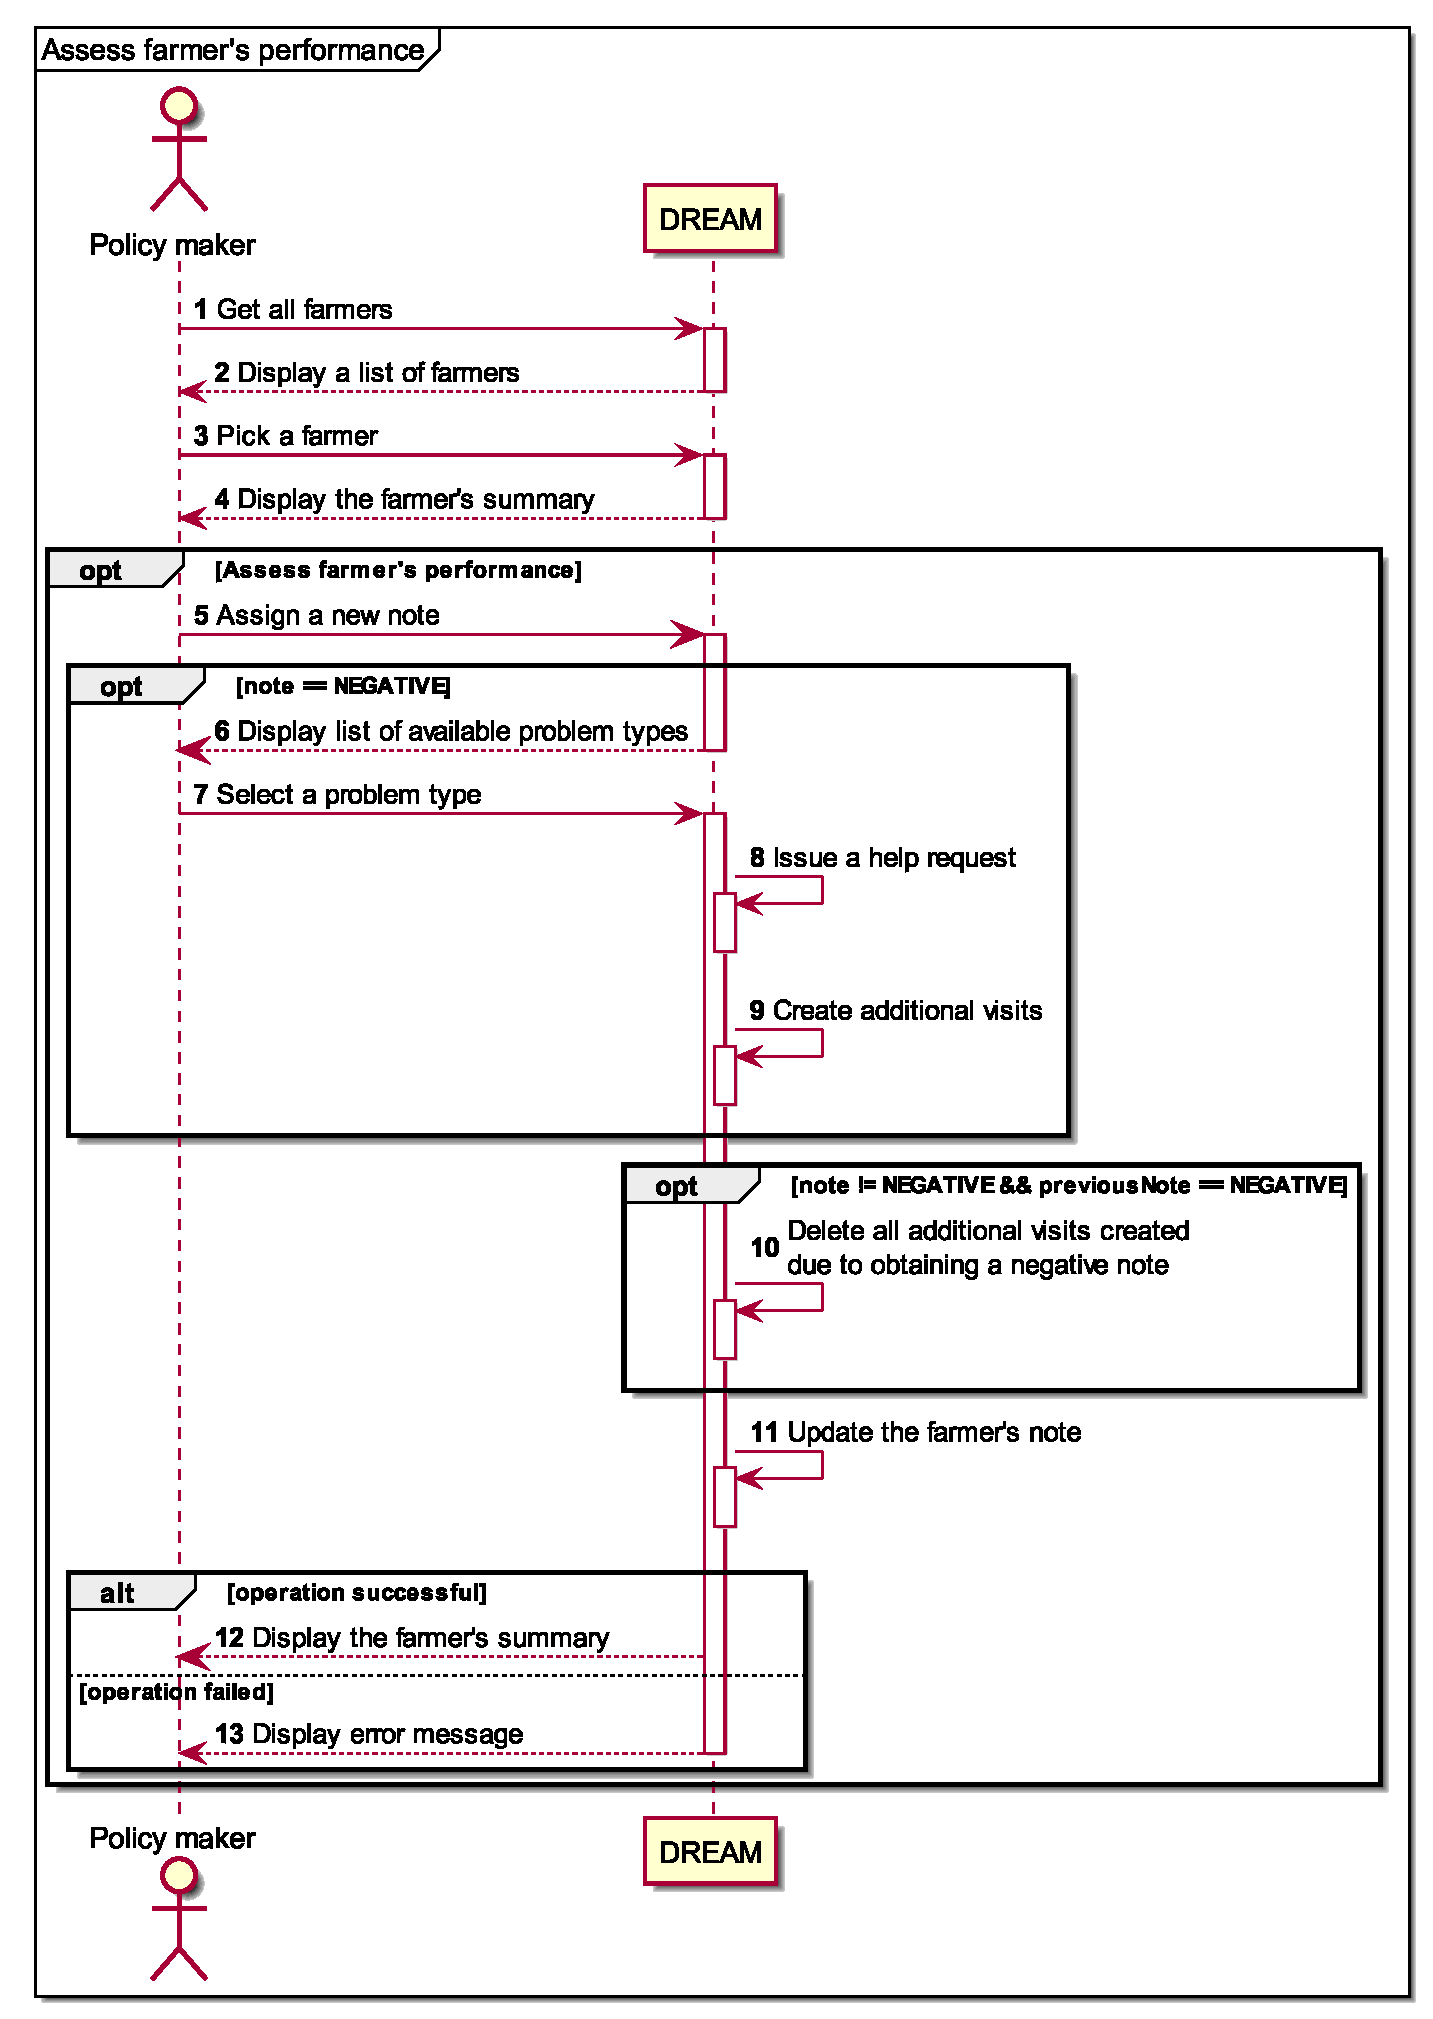
\includegraphics[scale=0.6, keepaspectratio, origin=c]{diagrams/sequence/assess_farmers_performance}
    \caption{Sequence diagram presenting farmer's performance assessment.}
    \label{fig:sd_assess_farmers_performance}
\end{figure}

\begin{table}[H]
    \centering
	\begin{tabular}{@{}p{0.25\linewidth} p{0.72\linewidth}@{}}
\toprule
		\textbf{Name}               & Create forum thread\\
		\midrule
		\textbf{Actors}             & Farmer\\
		\midrule
		\textbf{Goals}              & G6 \\
		\midrule
		
		\textbf{Entry conditions}   & \begin{itemize}[leftmargin=.4cm,noitemsep,topsep=0pt,before=\vspace{-3mm},after=\vspace{-4mm}]
		    \item The farmer is already logged in to the application.
		    \item The farmer is in the \textit{Forum} view, accessible from the sidebar of the application.
		\end{itemize}\\
		\midrule
		
		\textbf{Flow of events}     & \begin{enumerate}[leftmargin=.4cm,noitemsep,topsep=0pt,before=\vspace{-3mm},after=\vspace{-4mm}]
		    \item The farmer clicks on \textit{Create forum thread} at the bottom of the page.
		    \item The application shows a pop-up with textboxes to fill.
		    \item The farmer enters the topic and description of the thread.
		    \item The farmer clicks on \textit{Create} button.
		    \item The application creates a new forum thread.
		    \item The application displays the new thread.
		\end{enumerate}\\
		\midrule
		\textbf{Exit conditions}    & The application successfully created a new forum thread. From now on, the new forum thread is visible to all other farmers. User sees the new thread. \\
		\midrule
		
		\textbf{Exceptions}         & \begin{itemize}[leftmargin=.4cm,noitemsep,topsep=0pt,before=\vspace{-3mm}]
		   \item The farmer closes the pop-up showed in step 2 by clicking on a cross in the top right corner or the \textit{Cancel button} in the bottom.
		\end{itemize}
	    The system comes back to the \textit{Forum} view.
	    \begin{itemize}[leftmargin=.4cm,noitemsep,topsep=0pt]
		   \item The application is not able to create a forum thread in step 5. 
		\end{itemize}
		The application shows a message indicating a possible cause of the error.
        \\\bottomrule
	\end{tabular}
	\caption{Use case description: Create forum thread.} 
\end{table}

\begin{figure}[H]
    \centering
    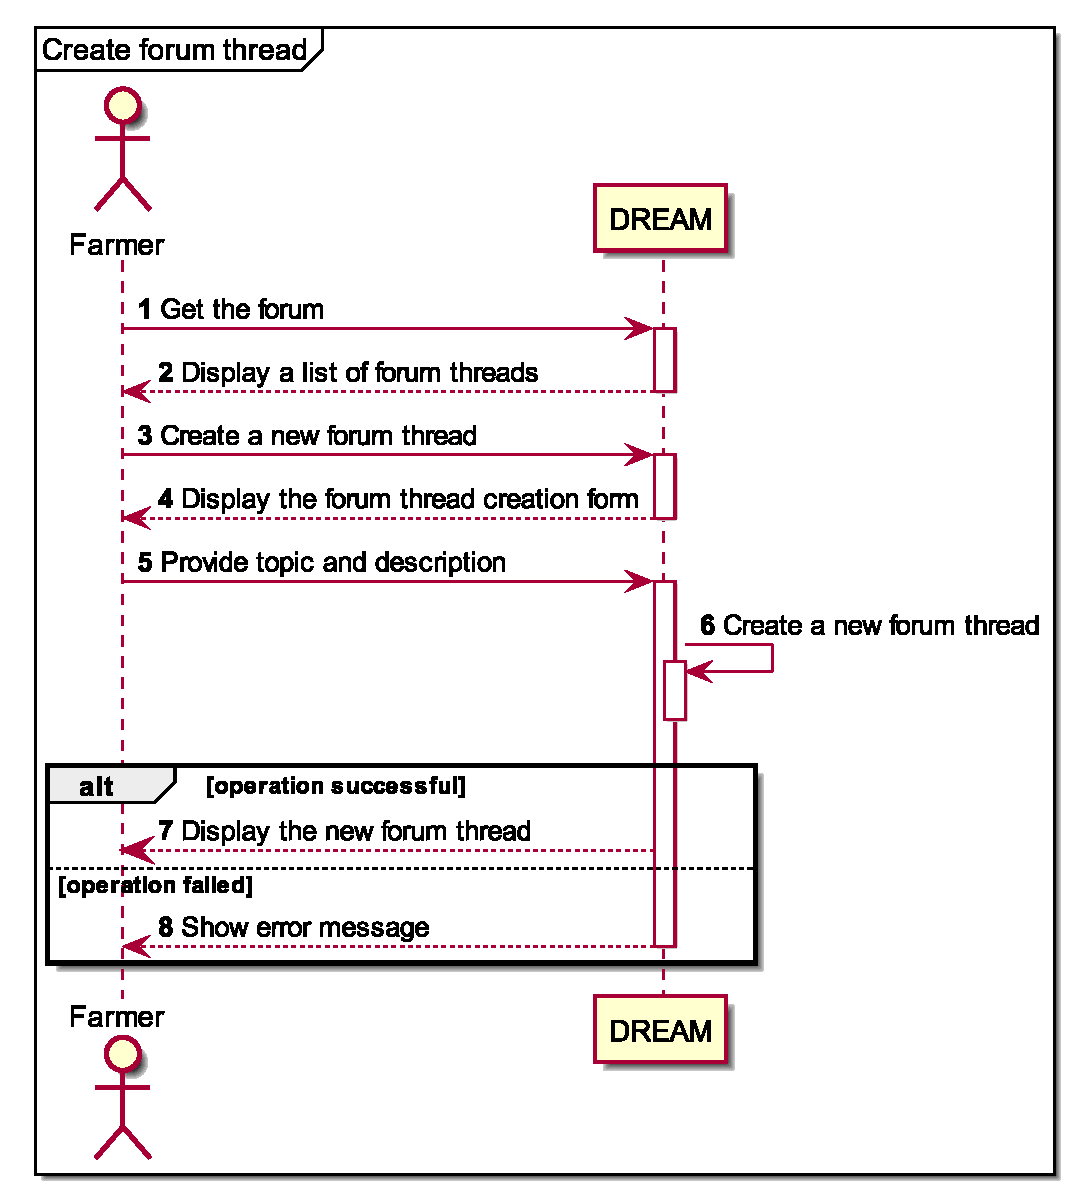
\includegraphics[scale=0.6, keepaspectratio, origin=c]{diagrams/sequence/create_forum_thread}
    \caption{Sequence diagram presenting the process of creating a new forum thread.}
    \label{fig:sd_create_forum_thread}
\end{figure}

\begin{table}[H]
    \centering
	\begin{tabular}{@{}p{0.25\linewidth} p{0.72\linewidth}@{}}
\toprule
		\textbf{Name}               & Add forum comment \\
		\midrule
		\textbf{Actors}             & Farmer\\
		\midrule
		\textbf{Goals}              & G6 \\
		\midrule
		
		\textbf{Entry conditions}   & \begin{itemize}[leftmargin=.4cm,noitemsep,topsep=0pt,before=\vspace{-3mm},after=\vspace{-4mm}]
		    \item The farmer is already logged in to the application.
		    \item The farmer is in the \textit{Forum} view, accessible from the sidebar of the application.
		\end{itemize}\\
		\midrule
		
		\textbf{Flow of events}     & \begin{enumerate}[leftmargin=.4cm,noitemsep,topsep=0pt,before=\vspace{-3mm},after=\vspace{-4mm}]
		    \item The farmer selects a forum thread, by clicking on the thread's topic in the list.
		    \item The application shows the contents of the selected forum thread.
		    \item The farmer fills the textbox with the content of his comment.
		    \item The farmer clicks on \textit{Send} button.
		    \item The application adds a new forum comment.
		    \item The application updates thread view, showing the new comment.
		\end{enumerate}\\
		\midrule
		\textbf{Exit conditions} & The application saved the new comment in the thread. From now on, the new comment is visible to all farmers viewing the thread. Farmer can see new comment in thread view. \\
		\midrule
		
		\textbf{Exceptions}         &
	    \begin{itemize}[leftmargin=.4cm,noitemsep,topsep=0pt]
		   \item The application is not able to add a forum comment in step 5. 
		\end{itemize}
		The application shows a message indicating a possible cause of the error.
		\\\bottomrule
	\end{tabular}
	\caption{Use case description: Add forum comment.} 
\end{table}

\begin{figure}[H]
    \centering
    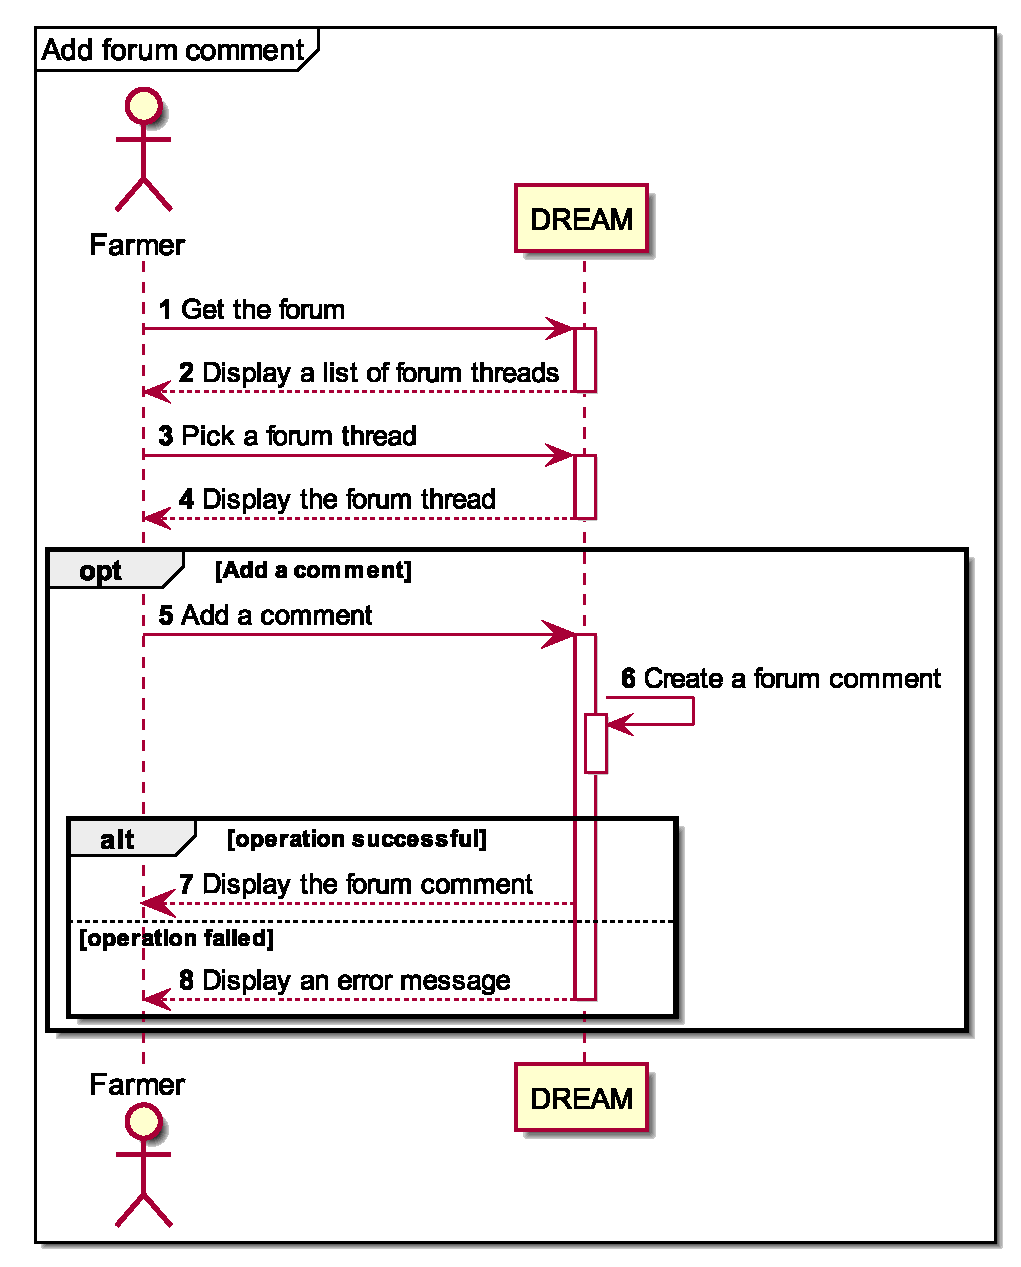
\includegraphics[scale=0.6, keepaspectratio, origin=c]{diagrams/sequence/add_forum_comment}
    \caption{Sequence diagram presenting the addition of a comment in a forum thread.}
    \label{fig:sd_add_forum_comment}
\end{figure}

\begin{table}[H]
    \centering
	\begin{tabular}{@{}p{0.25\linewidth} p{0.72\linewidth}@{}}
\toprule
		\textbf{Name}               & Display personal suggestions\\
		\midrule
		\textbf{Actors}             & Farmer\\
		\midrule
		\textbf{Goals}              & G1 \\
		\midrule
		
		\textbf{Entry conditions}   & \begin{itemize}[leftmargin=.4cm,noitemsep,topsep=0pt,before=\vspace{-3mm},after=\vspace{-4mm}]
		    \item The farmer is already logged in to the application.
		    \item The farmer is on the dashboard view.
		\end{itemize}\\
		\midrule
		
		\textbf{Flow of events}     & \begin{enumerate}[leftmargin=.4cm,noitemsep,topsep=0pt,before=\vspace{-3mm},after=\vspace{-4mm}]
		    \item The application shows personal suggestions on the top right part called \textit{Tips and suggestions} of the dashboard.
		    \item The farmer reads personal suggestions from the list.
		\end{enumerate}\\
		\midrule
		\textbf{Exit conditions}    & The farmer can read personalized suggestions showed in the dashboard view. \\
		\midrule
		
		\textbf{Exceptions}         & 
	    \begin{itemize}[leftmargin=.4cm,noitemsep,topsep=0pt,before=\vspace{-3mm}]
		   \item The application is not able to load personalized suggestions.
		\end{itemize}
		The application shows a message indicating a possible cause of the error.
		\\\bottomrule
	\end{tabular}
	\caption{Use case description: Display personal suggestions.} 
\end{table}


% \begin{table}[H]
%     \centering
% 	\begin{tabular}{@{}p{0.25\linewidth} p{0.72\linewidth}@{}}
% \toprule
% 		\textbf{Name}               & Visualize relevant data\\
% 		\midrule
% 		\textbf{Actors}             & Farmer\\
% 		\midrule
% 		\textbf{Goals}              & G1, G2 \\
% 		\midrule
		
% 		\textbf{Entry conditions}   & \begin{itemize}[leftmargin=.4cm,noitemsep,topsep=0pt,before=\vspace{-3mm},after=\vspace{-4mm}]
% 		    \item The farmer is already logged in to the application.
% 		    \item The farmer is on the dashboard view.
% 		\end{itemize}\\
% 		\midrule
		
% 		\textbf{Flow of events}     & \begin{enumerate}[leftmargin=.4cm,noitemsep,topsep=0pt,before=\vspace{-3mm},after=\vspace{-4mm}]
% 		    \item The user clicks on \textit{Relevant data} in the sidebar.
% 		    \item The application shows farmer's relevant data.
% 		\end{enumerate}\\
% 		\midrule
% 		\textbf{Exit conditions}    & The farmers is able to see the contents of farmer's relevant data. \\
% 		\midrule
		
% 		\textbf{Exceptions}         & 
% 	    \begin{itemize}[leftmargin=.4cm,noitemsep,topsep=0pt,before=\vspace{-3mm}]
% 		   \item The application is not able to load the farmer's relevant data.
% 		\end{itemize}
% 		The application shows a message indicating a possible cause of the error.
% 		\\\bottomrule
% 	\end{tabular}
% 	\caption{Use case description: visualize relevant data.} 
% \end{table}


\begin{table}[H]
    \centering
	\begin{tabular}{@{}p{0.25\linewidth} p{0.72\linewidth}@{}}
        \toprule
		\textbf{Name}               & View forum\\
		\midrule
		\textbf{Actors}             & Farmer\\
		\midrule
		\textbf{Goals}              & G6 \\
		\midrule
		
		\textbf{Entry conditions}   & \begin{itemize}[leftmargin=.4cm,noitemsep,topsep=0pt,before=\vspace{-3mm},after=\vspace{-4mm}]
		    \item The farmer is already logged in to the application.
		    \item The farmer is on the dashboard view.
		\end{itemize}\\
		\midrule
		
		\textbf{Flow of events}     & \begin{enumerate}[leftmargin=.4cm,noitemsep,topsep=0pt,before=\vspace{-3mm},after=\vspace{-4mm}]
		    \item The farmer clicks on \textit{Forum} in the sidebar.
		    \item The application shows the forum view with a list of already created forum threads.
		\end{enumerate}\\
		\midrule
		\textbf{Exit conditions}    & The farmer is able to see a list of already created forum threads. \\
		\midrule
		
		\textbf{Exceptions}         & 
	    \begin{itemize}[leftmargin=.4cm,noitemsep,topsep=0pt,before=\vspace{-3mm}]
		   \item The application is not able to load the list of already created forum threads.
		\end{itemize}
		The application shows a message indicating a possible cause of the error.
		\\\bottomrule
	\end{tabular}
	\caption{Use case description: View forum.} 
\end{table}

\begin{table}[H]
    \centering
	\begin{tabular}{@{}p{0.25\linewidth} p{0.72\linewidth}@{}}
        \toprule
		\textbf{Name}               & View forum thread\\
		\midrule
		\textbf{Actors}             & Farmer\\
		\midrule
		\textbf{Goals}              & G6 \\
		\midrule
		
		\textbf{Entry conditions}   & \begin{itemize}[leftmargin=.4cm,noitemsep,topsep=0pt,before=\vspace{-3mm},after=\vspace{-4mm}]
		    \item The farmer is already logged in to the application.
		    \item The farmer is on the forum view.
		\end{itemize}\\
		\midrule
		
		\textbf{Flow of events}     & \begin{enumerate}[leftmargin=.4cm,noitemsep,topsep=0pt,before=\vspace{-3mm},after=\vspace{-4mm}]
		    \item The farmer finds a forum thread he is interested to see in the list.
		    \item The farmer clicks on the forum thread he found in the previous step.
		    \item The application loads the contents of the selected forum thread.
		\end{enumerate}\\
		\midrule
		\textbf{Exit conditions}    &  The farmer is able to read the contents of the forum thread. \\
		\midrule
		
		\textbf{Exceptions}         & 
	    \begin{itemize}[leftmargin=.4cm,noitemsep,topsep=0pt,before=\vspace{-3mm}]
		   \item The application is not able to load the contents of the selected forum thread.
		\end{itemize}
		The application shows a message indicating a possible cause of the error.
		\\\bottomrule
	\end{tabular}
	\caption{Use case description: View forum.} 
\end{table}

\begin{table}[H]
    \centering
	\begin{tabular}{@{}p{0.25\linewidth} p{0.72\linewidth}@{}}
\toprule
		\textbf{Name}               & Request help\\
		\midrule
		\textbf{Actors}             & Farmer\\
		\midrule
		\textbf{Goals}              & G5, G6 \\
		\midrule
		
		\textbf{Entry conditions}   & \begin{itemize}[leftmargin=.4cm,noitemsep,topsep=0pt,before=\vspace{-3mm},after=\vspace{-4mm}]
		    \item The farmer is already logged in to the application.
		\end{itemize}\\
		\midrule
		
		\textbf{Flow of events}     & \begin{enumerate}[leftmargin=.4cm,noitemsep,topsep=0pt,before=\vspace{-3mm},after=\vspace{-4mm}]
		    \item The farmer clicks on \textit{My help requests} view in the sidebar.
		    \item The farmer clicks on \textit{Create help request} button.
		    \item The application shows a pop-up with textboxes to fill.
		    \item The farmer enters a topic and message.
		    \item The farmer clicks on \textit{Send request} button.
		    \item The application sends requests to the agronomists and several farmers with a positive note working in the given area. 
		    \item The application shows the created request.
		\end{enumerate}\\
		\midrule
		\textbf{Exit conditions}    & The request can be seen in the \textit{Provide help} view by the recipients selected in step 6. Additionally, the farmer who created the request can see it in the \textit{My help requests} view. \\
		\midrule
		
		\textbf{Exceptions}         & \begin{itemize}[leftmargin=.4cm,noitemsep,topsep=0pt,before=\vspace{-3mm}]
		   \item The farmer closes the pop-up showed in step 3 by clicking on \textit{Cancel} button or on a  cross in a top right corner.
		\end{itemize}
	    The system comes back to the \textit{My help requests} view.
	    \begin{itemize}[leftmargin=.4cm,noitemsep,topsep=0pt]
		   \item The application is not able to create a request for help in step 6. 
		\end{itemize}
		The application shows a message indicating a possible cause of the error.\\
		\bottomrule
	\end{tabular}
	\caption{Use case description: Request help.} 
\end{table}

\begin{figure}[H]
    \centering
    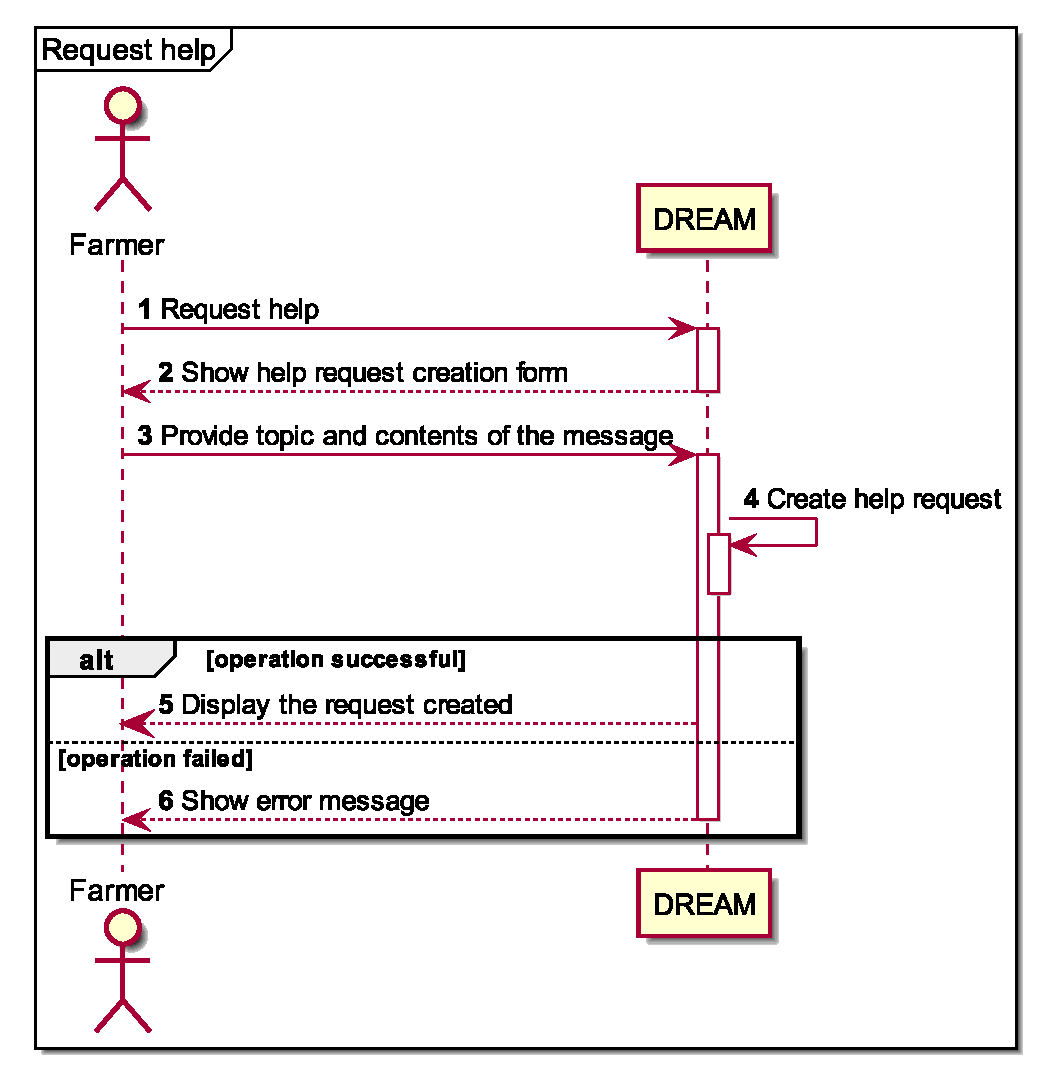
\includegraphics[scale=0.6, keepaspectratio, origin=c]{diagrams/sequence/request_help}
    \caption{Sequence diagram presenting the creation of a help request.}
    \label{fig:sd_request_help}
\end{figure}

\begin{table}[H]
    \centering
	\begin{tabular}{@{}p{0.25\linewidth} p{0.72\linewidth}@{}}
\toprule
		\textbf{Name}               & Create response\\
		\midrule
		\textbf{Actors}             & Agronomist, Farmer (positive note)\\
		\midrule
		\textbf{Goals}              & G5, G6 \\
		\midrule
		
		\textbf{Entry conditions}   & \begin{itemize}[leftmargin=.4cm,noitemsep,topsep=0pt,before=\vspace{-3mm},after=\vspace{-4mm}]
		    \item The farmer or the agronomist is already logged in to the application.
		    \item The farmer or the agronomist is in the \textit{Provide help} view.
		\end{itemize}\\
		\midrule
		
		\textbf{Flow of events}     & \begin{enumerate}[leftmargin=.4cm,noitemsep,topsep=0pt,before=\vspace{-3mm},after=\vspace{-4mm}]
		    \item The farmer or the agronomist clicks on the requests he wants to reply to. 
		    \item The application shows a pop-up with textboxes to fill.
		    \item The farmer or the agronomist enters the contents of the reply message.
		    \item The farmer or the agronomist clicks the \textit{Send} button.
		    \item The application saves the answer to the request.
		    \item The application shows a message indicating successful sending of the message.
		\end{enumerate}\\
		\midrule
		\textbf{Exit conditions}    & The farmer can see the response by clicking on the request in the \textit{My help request tab}. \\
		\midrule
		
		\textbf{Exceptions}         & 
	    \begin{itemize}[leftmargin=.4cm,noitemsep,topsep=0pt,before=\vspace{-3mm}]
		   \item The application is not able to create an answer to a help request in step 5. 
		\end{itemize}
		The application shows a message indicating a possible cause of the error.
		\begin{itemize}[leftmargin=.4cm,noitemsep,before=\vspace{-3mm}]
		   \item The user resigns from creating a response to the request by clicking on the cross in the top right corner or \textit{Cancel button}. 
		\end{itemize}
		The application comes back to \textit{Provide help} view.
		\\\bottomrule
	\end{tabular}
	\caption{Use case description: Create response.} 
\end{table}

\begin{figure}[H]
    \centering
    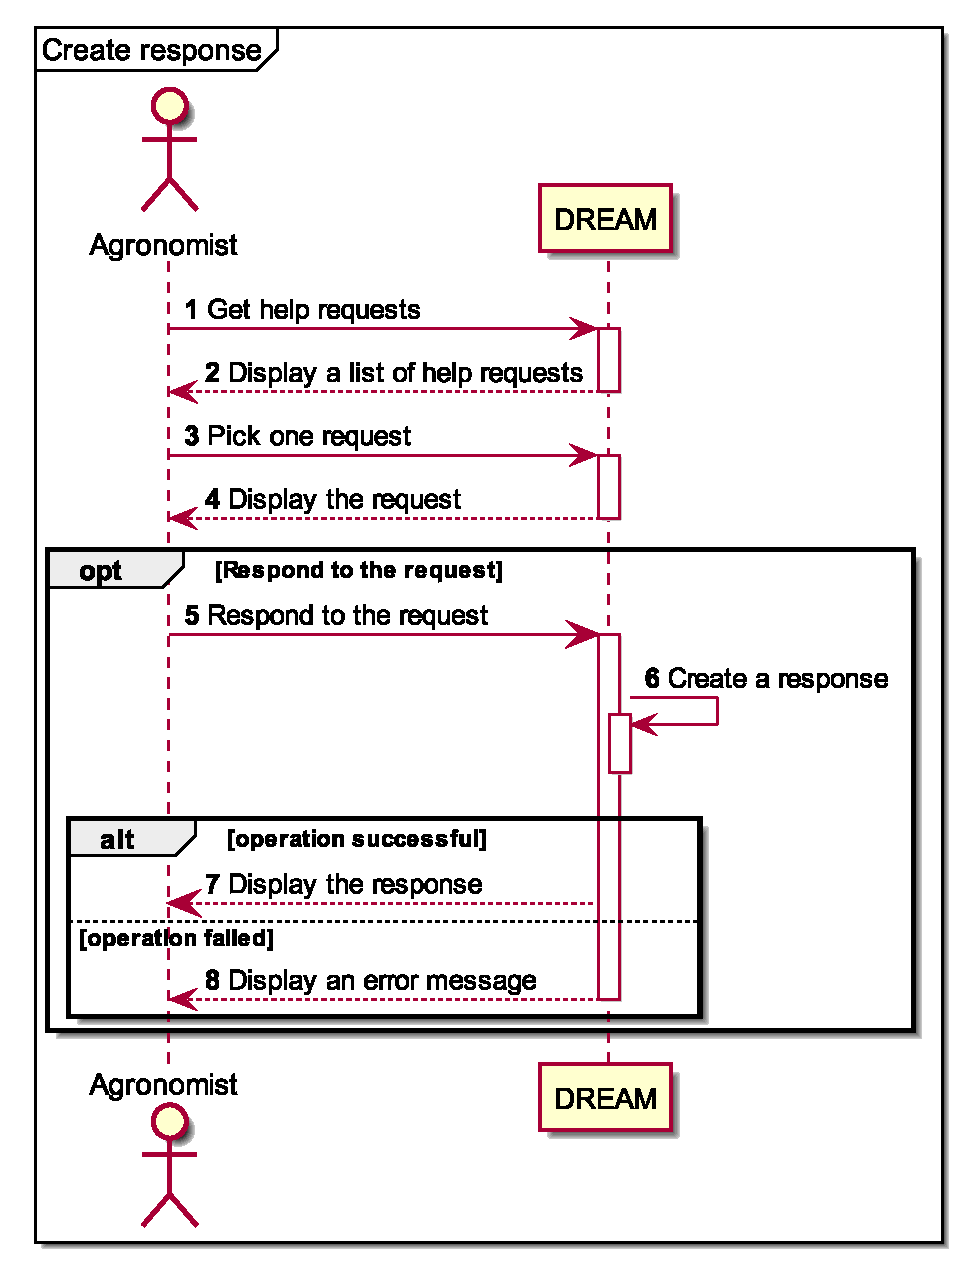
\includegraphics[scale=0.6, keepaspectratio, origin=c]{diagrams/sequence/create_response}
    \caption{Sequence diagram presenting the event of answering to a help request.}
    \label{fig:sd_create_response}
\end{figure}

\begin{table}[H]
    \centering
	\begin{tabular}{@{}p{0.25\linewidth} p{0.72\linewidth}@{}}
    \toprule
		\textbf{Name}               & View farmer's summary\\
		\midrule
		\textbf{Actors}             & Agronomist, Farmer, Policy maker\\
		\midrule
		\textbf{Goals}              & G2, G3, G5, G6 \\
		\midrule
		
		\textbf{Entry conditions}   & \begin{itemize}[leftmargin=.4cm,noitemsep,topsep=0pt,before=\vspace{-3mm},after=\vspace{-4mm}]
		    \item The user is already logged in to the application.
		    \item The user is on the dashboard view.
		\end{itemize}\\
		\midrule
		
		\textbf{Flow of events}     & \begin{enumerate}[leftmargin=.4cm,noitemsep,topsep=0pt,before=\vspace{-3mm},after=\vspace{-4mm}]
		    \item If the user is Agronomist or Policy Maker
		    \begin{enumerate}[noitemsep]
		        \item The user clicks on \textit{Farmers} in the sidebar.
		        \item The application shows a list of farmers.
		        \item The user finds in a list a farmer whose summary he wants to see.
		        \item The user clicks on an eye icon.
		    \end{enumerate}
		    \item If the user is Farmer
		    \begin{enumerate}[noitemsep]
		        \item The user clicks on \textit{Summary} in the sidebar.
		    \end{enumerate}
		    \item The application shows a farmer's summary page.
		\end{enumerate}\\
		\midrule
		\textbf{Exit conditions}    & The user is able to see the contents of farmer's summary. \\
		\midrule
		
		\textbf{Exceptions}         & 
	    \begin{itemize}[leftmargin=.4cm,noitemsep,topsep=0pt,before=\vspace{-3mm}]
		   \item The application is not able to load the farmer's summary of the selected farmer.
		\end{itemize}
		The application shows a message indicating a possible cause of the error.
		\\\bottomrule
	\end{tabular}
	\caption{Use case description: View farmer's summary.} 
\end{table}

\begin{table}[H]
    \centering
	\begin{tabular}{@{}p{0.25\linewidth} p{0.72\linewidth}@{}}
        \toprule
		\textbf{Name}               & View daily plan\\
		\midrule
		\textbf{Actors}             & Agronomist\\
		\midrule
		\textbf{Goals}              & G4 \\
		\midrule
		
		\textbf{Entry conditions}   & \begin{itemize}[leftmargin=.4cm,noitemsep,topsep=0pt,before=\vspace{-3mm},after=\vspace{-4mm}]
		    \item The agronomist is already logged in to the application.
		    \item The agronomist is on the dashboard view.
		\end{itemize}\\
		\midrule
		
		\textbf{Flow of events}     & \begin{enumerate}[leftmargin=.4cm,noitemsep,topsep=0pt,before=\vspace{-3mm},after=\vspace{-4mm}]
		    \item The agronomist clicks on \textit{Daily plan} in the sidebar.
		    \item The application shows daily plan view for the current day.
		\end{enumerate}\\
		\midrule
		\textbf{Exit conditions}    & The agronomist can see daily plan for the current day. The agronomist can choose another day from the calendar on the left side of the view. \\
		\midrule
		
		\textbf{Exceptions}         & 
	    \begin{itemize}[leftmargin=.4cm,noitemsep,topsep=0pt,before=\vspace{-3mm}]
		   \item The application is not able to load the daily plan of the agronomist.
		\end{itemize}
		The application shows a message indicating a possible cause of the error.
		\\\bottomrule
	\end{tabular}
	\caption{Use case description: View daily plan.} 
\end{table}

\begin{table}[H]
    \centering
	\begin{tabular}{@{}p{0.25\linewidth} p{0.72\linewidth}@{}}
		\toprule
		\textbf{Name}               & Set daily plan execution state \\
		\midrule
		\textbf{Actors}             & Agronomist\\
		\midrule
		\textbf{Goals}              & G4 \\
		\midrule
		
		\textbf{Entry conditions}   & \begin{itemize}[leftmargin=.4cm,noitemsep,topsep=0pt,before=\vspace{-3mm},after=\vspace{-4mm}]
		    \item The agronomist is already logged in to the application.
		    \item The agronomist is in the \textit{Daily plan} view.
		\end{itemize}\\
		\midrule
		
		\textbf{Flow of events}     & \begin{enumerate}[leftmargin=.4cm,noitemsep,topsep=0pt,before=\vspace{-3mm},after=\vspace{-4mm}]
		    \item The agronomist clicks on a day in the calendar for which execution state is to be set.
		    \item The agronomist clicks on \textit{Submit execution state} button.
		    \item The application shows a pop-up with a list of visits in a selected day.
		    \item The agronomist marks each checkbox next to the visits he has done, leaving unmarked checkboxes next to the visits he skipped.
		    \item The application shows text fields below each visit with marked checkbox.
		    \item The agronomist fills text fields shown in the previous step with comments he collected during the visits.
		    \item The agronomist clicks on \textit{Submit} button to save the execution state.
		    \item The application saves the execution state.
		    \item The application plans new visits to farms that were visited in terms of a casual visit in approximately half of a year.
		    \item The application plans new visits to the farms that were not visited, but should be visited in terms of a casual visit, in approximately the next 5 days.
		\end{enumerate}\\
		\midrule
		\textbf{Exit conditions}    & The state of visits for the given date is saved in the system. New visits are planned in dates depending on the state of the last visit (if it was \textit{confirmed} or \textit{rejected}). \\
		\midrule
		
		\textbf{Exceptions}         & \begin{itemize}[leftmargin=.4cm,noitemsep,topsep=0pt,before=\vspace{-3mm}]
		   \item The agronomist cancels the operation in the steps 3-6 by clicking on the \textit{Cancel} button or a cross in the top right corner of the pop-up.
		\end{itemize}
		The application comes back to the daily plan view.
	    \begin{itemize}[leftmargin=.4cm,noitemsep,topsep=0pt]
		   \item The application is not able to save the execution state in the step 8. 
		\end{itemize}
		The application shows a message indicating a possible cause of the error.
	    \\\bottomrule
	\end{tabular}
	\caption{Use case description: Set daily plan execution state.} 
\end{table}

\begin{figure}[H]
    \centering
    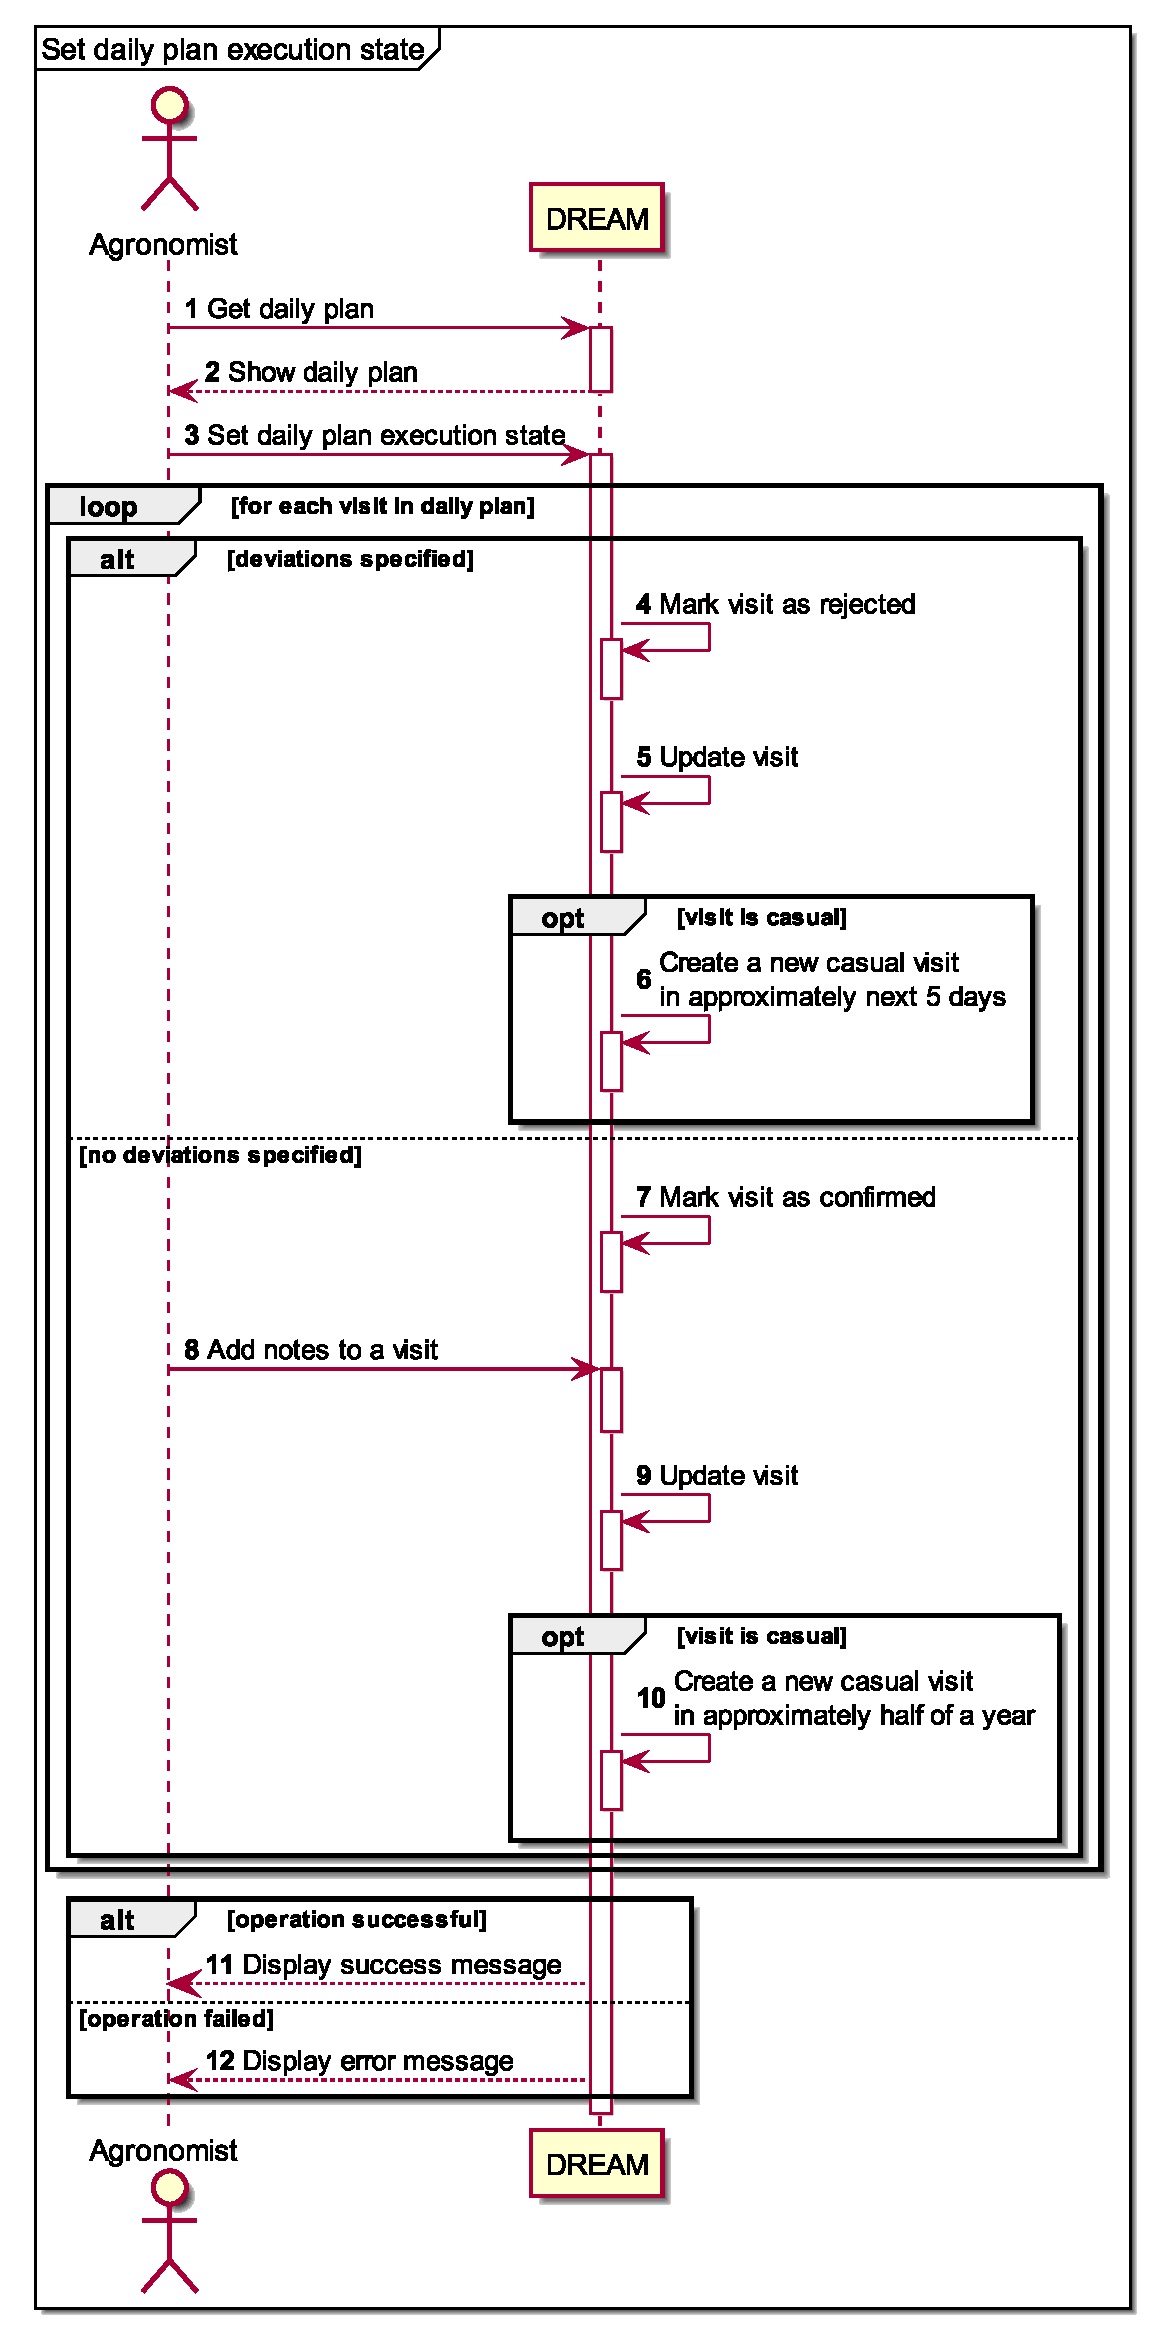
\includegraphics[scale=0.6, keepaspectratio, height=0.98\textheight, origin=c]{diagrams/sequence/set_daily_plan_execution_state}
    \caption{Sequence diagram presenting the action of displaying a daily plan.}
    \label{fig:sd_set_daily_plan_execution_state}
\end{figure}

\begin{table}[H]
    \centering
	\begin{tabular}{@{}p{0.25\linewidth} p{0.72\linewidth}@{}}
        \toprule
		\textbf{Name}               & Manage daily plan\\
		\midrule
		\textbf{Actors}             & Agronomist\\
		\midrule
		\textbf{Goals}              & G4 \\
		\midrule
		
		\textbf{Entry conditions}   & \begin{itemize}[leftmargin=.4cm,noitemsep,topsep=0pt,before=\vspace{-3mm},after=\vspace{-4mm}]
		    \item The agronomist is already logged in to the application.
		    \item The agronomist is in the daily plan view.
		\end{itemize}\\
		\midrule
		
		\textbf{Flow of events}     & \begin{enumerate}[leftmargin=.4cm,noitemsep,topsep=0pt,before=\vspace{-3mm},after=\vspace{-4mm}]
		    \item The agronomist clicks on the day in the calendar in which he wants to rearrange the visits.
		    \item The application shows a list of visits in the selected day.
		    \item The agronomist clicks on an edit icon to change the date of the selected visit.
		    \item The application shows a pop-up with a field to choose a new date for the visit.
		    \item The agronomist selects a new date for the visit selected in the previous step.
		    \item The agronomist confirms his choice.
		    \item The application saves changes made to the daily plan.
		    \item The application shows a message indicating successful save of the visit's date.
		\end{enumerate}\\
		\midrule
		\textbf{Exit conditions}    & The calendar in the \textit{Visit plan} view was modified accordingly. \\
		\midrule
		
		\textbf{Exceptions}         & \begin{itemize}[leftmargin=.4cm,noitemsep,topsep=0pt,before=\vspace{-3mm}]
		   \item An agronomist closes the pop-up shown in the step 4.
		\end{itemize}
	    The system shows the daily plan tab view. \begin{itemize}[leftmargin=.4cm,noitemsep,topsep=0pt]
		   \item An agronomist wants to delay a casual visit for more than 5 days.
		\end{itemize}
		The application shows an error, not allowing to delay the visit too much.
	    \begin{itemize}[leftmargin=.4cm,noitemsep,topsep=0pt]
		   \item The application is not able to save updates to the daily plan in step 6. 
		\end{itemize}
		The application shows a message indicating a possible cause of the error.
		\\\bottomrule
	\end{tabular}
	\caption{Use case description: Update daily plan.} 
\end{table}


\subsection{Mapping on requirements}

\begin{longtable}{p{0.06\linewidth} p{0.88\linewidth}} 
    \toprule
    \textbf{G1} & Improve farmers performance by providing them with personalized suggestions. \\ 
    \midrule
    \textbf{A5.} & Each farm is inside exactly one mandal.\\ 
    \textbf{A6.} & Each farmer reliably updates his production data each month.\\ 
    \textbf{A8.} & Agronomist's area of responsibility contains at least one mandal.\\ 
    \textbf{A10.} & The information provided by a user during registration process is valid.\\ 
    \textbf{A11.} & Well-performing farmers and agronomists are eager to help farmers with negative notes.\\ 
    \textbf{A12.} & Suggestions created by agronomists are relevant and helpful for the farmers. \\
    \textbf{A13.} & Each mandal has at least one agronomist who is responsible for the farms inside that area.\\ 
     
    %Requirements :C
    \midrule		
    %Authentication
	\textbf{R1.} & The system must uniquely identify each user by his e-mail. \\
	\textbf{R2.} & The system must allow an unregistered user to create an account with a chosen role. \\
	\textbf{R3.} & The system must ensure that an agronomist chooses the area of responsibility during the registration process. \\
	\textbf{R4.} & The system must ensure that a farmer inserts his farm data during the registration process.\\
	\textbf{R6.} & The system must allow a registered user to log in to the application. \\
	\textbf{R7.} & The system must allow a registered user to reset his password. \\
	\textbf{R8.} & The system must allow a logged-in user to sign out of the application. \\
	\textbf{R9.} & The system must allow a registered user to delete his account. \\
	
	%Farmer
	\textbf{R25.} & The system must allow a farmer to see personalized suggestions.\\
	\textbf{R26.} & The system must allow a farmer to manage his monthly production data.\\
	
	%Agronomist
	\textbf{R44.} & The system must allow an agronomist to manage his area of responsibility.\\
	\textbf{R45.} & The system must allow an agronomist to see the list of suggestions for mandals in his area of responsibility.\\
	\textbf{R46.} & The system must allow an agronomist to manage the list of suggestions for mandals in his area of responsibility.\\
	
    \bottomrule
    \caption{G1 mapping on assumptions and requirements.}
\end{longtable}

\begin{longtable}{p{0.06\linewidth} p{0.88\linewidth}} 
    \toprule
    \textbf{G2} & Acquire, combine, and visualize data from external systems. \\ 
    \midrule
    \textbf{A3.} & Each farm has at least one humidity sensor.\\ 
    \textbf{A4.} & Each farm has a water irrigation system.\\ 
    \textbf{A5.} & Each farm is inside exactly one mandal.\\ 
    \textbf{A7.} & Weather is consistent in a given mandal.\\ 
    \textbf{A10.} & The information provided by a user during registration process is valid.\\ 
    \textbf{A17.} & External systems are reliable and highly available.\\
    \textbf{A18.} & Every sensor system has a unique ID assigned by the sensor system provider. \\
    \textbf{A19.} & Every water irrigation system has a unique ID assigned by the water irrigation system provider. \\
    
    \midrule
    %Authentication
	\textbf{R1.} & The system must uniquely identify each user by his e-mail. \\
	\textbf{R2.} & The system must allow an unregistered user to create an account with a chosen role. \\
	\textbf{R3.} & The system must ensure that an agronomist chooses the area of responsibility during the registration process. \\
	\textbf{R4.} & The system must ensure that a farmer inserts his farm data during the registration process.\\
	\textbf{R5.} & The system must ensure that two casual farm visits are scheduled for each year of the farm's existence.\\
	\textbf{R6.} & The system must allow a registered user to log in to the application. \\
	\textbf{R7.} & The system must allow a registered user to reset his password. \\
	\textbf{R8.} & The system must allow a logged-in user to sign out of the application. \\
	\textbf{R9.} & The system must allow a registered user to delete his account. \\
	
	%Policy maker
	\textbf{R23.} & The system must allow a policy maker to see a farmer's summary.\\
	
	%Farmer
	\textbf{R24.} & The system must allow a farmer to see his own farmer's summary.\\
	\textbf{R37.} & The farmer is able to see farmer's summary of a farmer with a negative note whose help request he received. \\

	%Agronomist
	\textbf{R51.} & The system must allow an agronomist to see a farmer's summary in his area of responsibility.\\

    %External systems
	\textbf{R65.} & The system must read and update weather forecasts every day. \\
	\textbf{R66.} & The system must read and store data from humidity sensors every day. \\
	\textbf{R67.} & The system must read and store data from water irrigation systems every day. \\
    \bottomrule
    \caption{G2 mapping on assumptions and requirements.}
\end{longtable}

\begin{longtable}{p{0.06\linewidth} p{0.88\linewidth}} 
    \toprule
    \textbf{G3} & Facilitate performance assessment of the farmers. \\ 
    \midrule
    \textbf{A1.} & Each farmer possess exactly one farm.\\
    \textbf{A2.} & Each farm belongs to exactly one farmer.\\ 
    \textbf{A3.} & Each farm has at least one humidity sensor.\\ 
    \textbf{A4.} & Each farm has a water irrigation system.\\ 
    \textbf{A6.} & Each farmer reliably updates his production data each month.\\ 
    \textbf{A7.} & Weather is consistent in a given mandal.\\     
    \textbf{A9.} & Each registered user can be only one of the actors: an agronomist, a farmer, or a policy maker.\\ 
    \textbf{A10.} & The information provided by a user during registration process is valid.\\ 
    \textbf{A14.} & Based on the farmer's summary, a policy maker is able to understand whether the help given by farmers and agronomists produces significant results.\\ 
    \textbf{A17.} & External systems are reliable and highly available.\\
    \midrule
    
    %Authentication
	\textbf{R1.} & The system must uniquely identify each user by his e-mail. \\
	\textbf{R2.} & The system must allow an unregistered user to create an account with a chosen role. \\
	\textbf{R3.} & The system must ensure that an agronomist chooses the area of responsibility during the registration process. \\
	\textbf{R4.} & The system must ensure that a farmer inserts his farm data during the registration process.\\
	\textbf{R5.} & The system must ensure that two casual farm visits are scheduled for each year of the farm's existence.\\
	\textbf{R6.} & The system must allow a registered user to log in to the application. \\
	\textbf{R7.} & The system must allow a registered user to reset his password. \\
	\textbf{R8.} & The system must allow a logged-in user to sign out of the application. \\
	\textbf{R9.} & The system must allow a registered user to delete his account. \\
	
	%Policy maker
	\textbf{R10.} & The system must allow a policy maker to assign a note to a farmer.\\
	\textbf{R11.} & The system must ensure that every farmer initially has a neutral note.\\
	\textbf{R12.} & The system must have a list of predefined farmer's problem types.\\
    \textbf{R13.} & The system must allow a policy maker to specify a problem type when assigning a negative note.\\
	\textbf{R19.} & The system must allow a policy maker to see a list of all farmers in Telangana.\\
	\textbf{R20.} & The system must allow a policy maker to see a list of all farmers with a specific note.\\
	\textbf{R21.} & The system must allow a policy maker to see a list of all farmers in a given mandal.\\
	\textbf{R22.} & The system must allow a policy maker to find a farmer's summary by his name and surname.\\
	\textbf{R23.} & The system must allow a policy maker to see a farmer's summary.\\
	
    \bottomrule
\caption{G3 mapping on assumptions and requirements.}
\end{longtable}


\begin{longtable}{p{0.06\linewidth} p{0.88\linewidth}} 
    \toprule
    \textbf{G4} & Promote regular farms’ visits by agronomists. \\ 
    \midrule
    \textbf{A1.} & Each farmer possess exactly one farm.\\
    \textbf{A2.} & Each farm belongs to exactly one farmer.\\ 
    \textbf{A5.} & Each farm is inside exactly one mandal.\\ 
    \textbf{A8.} & Agronomist's area of responsibility contains at least one mandal.\\ 
    \textbf{A10.} & The information provided by a user during registration process is valid.\\ 
    \textbf{A11.} & Well-performing farmers and agronomists are eager to help farmers with negative notes.\\ 
    \textbf{A13.} & Each mandal has at least one agronomist who is responsible for the farms inside that area.\\ 
    \midrule
    
    %Authentication
	\textbf{R1.} & The system must uniquely identify each user by his e-mail. \\
	\textbf{R2.} & The system must allow an unregistered user to create an account with a chosen role. \\
	\textbf{R3.} & The system must ensure that an agronomist chooses the area of responsibility during the registration process. \\
	\textbf{R4.} & The system must ensure that a farmer inserts his farm data during the registration process.\\
	\textbf{R5.} & The system must ensure that two casual farm visits are scheduled for each year of the farm's existence.\\
	\textbf{R6.} & The system must allow a registered user to log in to the application. \\
	\textbf{R7.} & The system must allow a registered user to reset his password. \\
	\textbf{R8.} & The system must allow a logged-in user to sign out of the application. \\
	\textbf{R9.} & The system must allow a registered user to delete his account. \\
	
	%Policy maker
	\textbf{R10.} & The system must allow a policy maker to assign a note to a farmer.\\
	\textbf{R11.} & The system must ensure that every farmer initially has a neutral note.\\
	\textbf{R12.} & The system must have a list of predefined farmer's problem types.\\
    \textbf{R13.} & The system must allow a policy maker to specify a problem type when assigning a negative note.\\
    \textbf{R14.} & The system must ensure that a farm is visited more often in the event of any problems.\\
    \textbf{R15.} & The system must have a specified number of additional visits caused by each predefined problem type.\\
    \textbf{R16.} & The system must ensure that only the most recently specified problem type is taken into account when determining the number of visits.\\
	\textbf{R17.} & The system must ensure that an automatic help request followed by additional farm visits are created, if a farmer receives a negative note.\\
	\textbf{R18.} & The system must ensure that all the additional farm visits created due to obtaining a negative note are deleted after a farmer's negative note is updated with a positive or a neutral one.\\
	
	%Agronomist
	\textbf{R44.} & The system must allow an agronomist to manage his area of responsibility.\\
	\textbf{R57.} & The system must allow an agronomist to see his daily plans.\\
	\textbf{R58.} & The system must allow an agronomist to submit a daily plan's execution state, by rejecting or confirming each visit, on the same date or after the daily plan's date has passed. \\
	\textbf{R59.} & The system must allow an agronomist to provide a comment for a visit he is confirming.\\
	\textbf{R60.} & The system must ensure that after an agronomist submits his daily plan, for all the causal visits marked as confirmed, new ones are created in approximately half of a year.\\
	\textbf{R61.} & The system must allow an agronomist to delete a visit before its date.\\
	\textbf{R62.} & The system must ensure that a deleted visit is marked as rejected.\\
	\textbf{R63.} & The system must ensure that in case of rejecting a casual visit, a new one is created in maximally 5 days.\\
	\textbf{R64.} & The system must allow replanning any different visit than a casual one without any constraints.\\
    
    \bottomrule
    \caption{G4 mapping on assumptions and requirements.}
\end{longtable}
    

\begin{longtable}{p{0.06\linewidth} p{0.88\linewidth}} 
    \toprule
    \textbf{G5} & Enable agronomists to exchange information with farmers. \\ 
    \midrule
    \textbf{A5.} & Each farm is inside exactly one mandal.\\ 
    \textbf{A8.} & Agronomist's area of responsibility contains at least one mandal.\\ 
    \textbf{A10.} & The information provided by a user during registration process is valid.\\ 
    \textbf{A11.} & Well-performing farmers and agronomists are eager to help farmers with negative notes.\\ 
    \textbf{A13.} & Each mandal has at least one agronomist who is responsible for the farms inside that area.\\ 
    \textbf{A16.} & Farmers and agronomists create meaningful and not offensive help requests and responses. \\
    \midrule
    
	%Authentication
	\textbf{R1.} & The system must uniquely identify each user by his e-mail. \\
	\textbf{R2.} & The system must allow an unregistered user to create an account with a chosen role. \\
	\textbf{R3.} & The system must ensure that an agronomist chooses the area of responsibility during the registration process. \\
	\textbf{R4.} & The system must ensure that a farmer inserts his farm data during the registration process.\\
	\textbf{R5.} & The system must ensure that two casual farm visits are scheduled for each year of the farm's existence.\\
	\textbf{R6.} & The system must allow a registered user to log in to the application. \\
	\textbf{R7.} & The system must allow a registered user to reset his password. \\
	\textbf{R8.} & The system must allow a logged-in user to sign out of the application. \\
	\textbf{R9.} & The system must allow a registered user to delete his account. \\
	
	%Policy maker
    \textbf{R17.} & The system must ensure that an automatic help request followed by additional farm visits are created, if a farmer receives a negative note.\\
	
	%Farmer
	\textbf{R27.} & The system must allow a farmer to see a list of help requests created by him.\\
	\textbf{R28.} & The system must allow a farmer to find a help request created by him by the topic.\\
	\textbf{R29.} & The system must allow a farmer to see a specific help request created by him.\\
	\textbf{R30.} & The system must allow a farmer to delete a specific help request created by him.\\
	\textbf{R31.} & The system must allow a farmer to create a new help request.\\
	
	%Agronomist
	\textbf{R44.} & The system must allow an agronomist to manage his area of responsibility.\\
	\textbf{R47.} & The system must allow an agronomist to see a list of all farmers in his area of responsibility.\\
	\textbf{R48.} & The system must allow an agronomist to see a list of all farmers with a specific note in his area of responsibility.\\
	\textbf{R49.} & The system must allow an agronomist to see a list of all farmers in a given mandal in his area of responsibility.\\
	\textbf{R50.} & The system must allow an agronomist to find a farmer's summary in his area of responsibility by his name and surname.\\
	\textbf{R51.} & The system must allow an agronomist to see a farmer's summary in his area of responsibility.\\
	\textbf{R52.} & The system must allow an agronomist to see a list of all help requests in his area of responsibility.\\
	\textbf{R53.} & The system must allow an agronomist to find a help request in his area of responsibility by the topic.\\
	\textbf{R54.} & The system must allow an agronomist to see a specific help request in his area of responsibility.\\
	\textbf{R55.} & The system must allow an agronomist to respond to a specific help request in his area of responsibility.\\
	\textbf{R56.} & The system must allow an agronomist to delete a help response, only if it was created by him.\\

    \bottomrule
    \caption{G5 mapping on assumptions and requirements.}
\end{longtable}

\begin{longtable}{p{0.06\linewidth} p{0.88\linewidth}} 
    \toprule
    \textbf{G6} & Enable farmers to exchange their knowledge. \\ 
    \midrule
    \textbf{A10.} & The information provided by a user during registration process is valid.\\ 
    \textbf{A11.} & Well-performing farmers and agronomists are eager to help farmers with negative notes.\\ 
    \textbf{A15.} & Farmers create meaningful and not offensive threads and comments on the forum.\\ 
    \textbf{A16.} & Farmers and agronomists create meaningful and not offensive help requests and responses. \\
    \midrule
    
    %Authentication
	\textbf{R1.} & The system must uniquely identify each user by his e-mail. \\
	\textbf{R2.} & The system must allow an unregistered user to create an account with a chosen role. \\
	\textbf{R3.} & The system must ensure that an agronomist chooses the area of responsibility during the registration process. \\
	\textbf{R4.} & The system must ensure that a farmer inserts his farm data during the registration process.\\
	\textbf{R5.} & The system must ensure that two casual farm visits are scheduled for each year of the farm's existence.\\
	\textbf{R6.} & The system must allow a registered user to log in to the application. \\
	\textbf{R7.} & The system must allow a registered user to reset his password. \\
	\textbf{R8.} & The system must allow a logged-in user to sign out of the application. \\
	\textbf{R9.} & The system must allow a registered user to delete his account. \\
	
	%Policy maker
    \textbf{R17.} & The system must ensure that an automatic help request followed by additional farm visits are created, if a farmer receives a negative note.\\
	
	%Farmer
	\textbf{R27.} & The system must allow a farmer to see a list of help requests created by him.\\
	\textbf{R28.} & The system must allow a farmer to find a help request created by him by the topic.\\
	\textbf{R29.} & The system must allow a farmer to see a specific help request created by him.\\
	\textbf{R30.} & The system must allow a farmer to delete a specific help request created by him.\\
	\textbf{R31.} & The system must allow a farmer to create a new help request.\\
	\textbf{R32.} & The system must allow a farmer with a positive note to see a list of all help requests in his mandal.\\
	\textbf{R33.} & The system must allow a farmer with a positive note to find a help request in his mandal by the topic.\\
	\textbf{R34.} & The system must allow a farmer with a positive note to see a specific help request in his mandal.\\
	\textbf{R35.} & The system must allow a farmer with a positive note to respond to a specific help request in his mandal.\\
	\textbf{R36.} & The system must allow a farmer with a positive note to delete a help response, only if it was created by him.\\
	\textbf{R37.} & The farmer is able to see farmer's summary of a farmer with a negative note whose help request he received. \\
	\textbf{R38.} & The system must allow a farmer to see a list of all forum threads in Telangana.\\
	\textbf{R39.} & The system must allow a farmer to find a forum thread by the topic.\\
	\textbf{R40.} & The system must allow a farmer to see a specific forum thread with its comments.\\
	\textbf{R41.} & The system must allow a farmer to create a comment in a forum thread.\\
	\textbf{R42.} & The system must allow a farmer to delete a comment in a forum thread, only if it was created by him.\\
	\textbf{R43.} & The system must allow a farmer to create a forum thread.\\
	
    \bottomrule
    \caption{G6 mapping on assumptions and requirements.}
\end{longtable}

\section{Performance Requirements} \label{sec:performance_requirements}

Given that the system is intended for Telangana farmers, agronomists, and policymakers, it is fair to assume that it will be utilized by about 30 000 people. Therefore, the following performance requirements, which were formulated taking into consideration the best practices \cite{performance_requirements}, should be met.

\subsection{Response Time}

\begin{itemize}
    \item During peak hours, the average response time should be 2 seconds.
    \item During peak hours, 99\% of all response times must be shorter than 3 seconds.
    \item In each 10-minute period commencing on the hour, the average response time must be 2 seconds or less.
    \item 95\% percent of all response times must be shorter than 2 seconds.
\end{itemize}
 
\subsection{Workload}

\begin{itemize}
    \item The system must be capable of processing 20 transactions per second.
    \item The system must have no more than one hour of downtime every three months.
\end{itemize}

\subsection{Scalability}

\begin{itemize}
    \item The system must be able to sustain a 5\% yearly growth in new users.
    \item The system must be able to sustain a 10\% yearly increase in the number of transactions per second.
    \item The system shall be able to extend its connections to new external systems providing relevant data as their number may arise.
\end{itemize}

\subsection{Platform}

DREAM has to be housed on a platform that meets the following criteria:

\begin{itemize}
    \item Operating system: Windows 10 or Windows 11.    
    \item \textit{.NET 6.0} development platform installed.
    \item \textit{PostgreSQL} object-relational database system.
    \item CPU: 1.4 GHz 64-bit processor compatible with x64 instruction set.
    \item Memory: Minimum 8 GB of RAM. 
    \item Hard drive space: minimum of 20 GB of space.
    \item Network adapter: an Ethernet adapter capable of at least 1 gigabit per second throughput.
\end{itemize}

\section{Design Constraints}

This section describes the constraints of a design. These include uncontrolled limitations that are self-imposed in order to enhance the design.

\subsection{Standards compliance}

The system will collect data from external systems and sensors, as well as data entered by users during registration and application use, such as production data, agronomist's daily plan, farmer's summary, and notes. The data will be used exclusively for system purposes and will be treated discreetly in accordance with the General Data Protection Regulation \cite{GDPR} and IS 17428.1 \cite{india_privacy_doc} guidelines. In particular, no information relating to a specific person will be made public as a result of the statistical analyses undertaken.

\subsection{Hardware limitations}

The following are the hardware constraints that the end user must meet in order to use the system.

\begin{itemize}
    \item Processor: 1.9 GHz x86- or x64-bit dual-core processor.
    \item Memory: 2 GB of RAM.
    \item Network: wired or wireless connection with bandwidth greater than 40 KBps (320 kbps) and latency under 200 ms.
    \item Web browser: Google Chrome, Firefox, Safari, Microsoft Edge, or Opera running on Windows, macOS, Linux, or mobile operating systems including Android and iOS, with \textit{JavaScript} enabled.
\end{itemize}

\subsection{Any other constraints}

DREAM will employ stateless protocols to enable components to be handled and changed without impacting the overall system. Additionally, the system will catalog, retrieve and run queries on all the relevant data using a relational database.

\section{Software System Attributes}

The system's characteristics that facilitate the measurement of its performance are presented in this section.

\subsection{Reliability}

The mean time between failures shall be equal to 120 hours, which means that in the worst case scenario it may break once every 5 days. Furthermore, the system shall be fault-tolerant, with its architecture prepared for any potential damage to system components by having replicas ready to be substituted. In order to recover from eventual data losses, redundancy should be considered for the system's database implementation.

\subsection{Availability}

As mentioned in the section \ref{sec:performance_requirements}, the system shall have no more than one hour of downtime every three months, thus, shall be highly available. In case of any planned maintenance works, all the users should be notified at least 48 hours in advance.

\subsection{Security}

The system shall implement role-based access control, which is a method of restricting system access to authorized users and granting permissions based on the user's role. It is accomplished through the use of both authentication and authorization implemented in the backend. The former is based on verifying the identity of a user, which can be an agronomist, a farmer, or a policy maker, during the log in phase. The latter, on the other hand, validates the logged-in user's permissions to perform an action (for example, visualizing an agronomist's daily plan) before actually carrying it out.

\subsection{Maintainability}

The system shall be written in a widely known programming language, which would ensure a high level of maintainability and a relatively simple induction for potential new members of the development team. Following that, it should be divided into modularized components to ease replacements and fixes in the event of a failure. The system's backend must be capable of supporting maintenance works on a copy, which will subsequently be deployed after being tested on pre-defined test suites, in order to ensure no downtime for the core functionalities.

Both the testing scenarios and the tests themselves should be defined. This contains both end-to-end testing and basic unit tests. The code coverage should then be monitored and controlled. In the event of a system failure, thorough crash reports must be sent to the developers.

Maintenance pauses will be arranged on occasion throughout the night, when user traffic is at its lowest.

\subsection{Portability}

DREAM will be offered as a web application, making it available on the vast majority of current web browsers, including desktop and mobile machines. Because of this approach, the system will be usable on a wide range of devices. User interface adjustments shall be made to make the application user-friendly on all the environments.
